% Options for packages loaded elsewhere
\PassOptionsToPackage{unicode}{hyperref}
\PassOptionsToPackage{hyphens}{url}
%
\documentclass[
  11pt,
]{article}
\usepackage{amsmath,amssymb}
\usepackage{lmodern}
\usepackage{iftex}
\ifPDFTeX
  \usepackage[T1]{fontenc}
  \usepackage[utf8]{inputenc}
  \usepackage{textcomp} % provide euro and other symbols
\else % if luatex or xetex
  \usepackage{unicode-math}
  \defaultfontfeatures{Scale=MatchLowercase}
  \defaultfontfeatures[\rmfamily]{Ligatures=TeX,Scale=1}
\fi
% Use upquote if available, for straight quotes in verbatim environments
\IfFileExists{upquote.sty}{\usepackage{upquote}}{}
\IfFileExists{microtype.sty}{% use microtype if available
  \usepackage[]{microtype}
  \UseMicrotypeSet[protrusion]{basicmath} % disable protrusion for tt fonts
}{}
\makeatletter
\@ifundefined{KOMAClassName}{% if non-KOMA class
  \IfFileExists{parskip.sty}{%
    \usepackage{parskip}
  }{% else
    \setlength{\parindent}{0pt}
    \setlength{\parskip}{6pt plus 2pt minus 1pt}}
}{% if KOMA class
  \KOMAoptions{parskip=half}}
\makeatother
\usepackage{xcolor}
\IfFileExists{xurl.sty}{\usepackage{xurl}}{} % add URL line breaks if available
\IfFileExists{bookmark.sty}{\usepackage{bookmark}}{\usepackage{hyperref}}
\hypersetup{
  pdftitle={Quantifying Stability and Change in Personal Culture Using Panel Data},
  hidelinks,
  pdfcreator={LaTeX via pandoc}}
\urlstyle{same} % disable monospaced font for URLs
\usepackage[margin=1in]{geometry}
\usepackage{graphicx}
\makeatletter
\def\maxwidth{\ifdim\Gin@nat@width>\linewidth\linewidth\else\Gin@nat@width\fi}
\def\maxheight{\ifdim\Gin@nat@height>\textheight\textheight\else\Gin@nat@height\fi}
\makeatother
% Scale images if necessary, so that they will not overflow the page
% margins by default, and it is still possible to overwrite the defaults
% using explicit options in \includegraphics[width, height, ...]{}
\setkeys{Gin}{width=\maxwidth,height=\maxheight,keepaspectratio}
% Set default figure placement to htbp
\makeatletter
\def\fps@figure{htbp}
\makeatother
\setlength{\emergencystretch}{3em} % prevent overfull lines
\providecommand{\tightlist}{%
  \setlength{\itemsep}{0pt}\setlength{\parskip}{0pt}}
\setcounter{secnumdepth}{-\maxdimen} % remove section numbering
\newlength{\cslhangindent}
\setlength{\cslhangindent}{1.5em}
\newlength{\csllabelwidth}
\setlength{\csllabelwidth}{3em}
\newlength{\cslentryspacingunit} % times entry-spacing
\setlength{\cslentryspacingunit}{\parskip}
\newenvironment{CSLReferences}[2] % #1 hanging-ident, #2 entry spacing
 {% don't indent paragraphs
  \setlength{\parindent}{0pt}
  % turn on hanging indent if param 1 is 1
  \ifodd #1
  \let\oldpar\par
  \def\par{\hangindent=\cslhangindent\oldpar}
  \fi
  % set entry spacing
  \setlength{\parskip}{#2\cslentryspacingunit}
 }%
 {}
\usepackage{calc}
\newcommand{\CSLBlock}[1]{#1\hfill\break}
\newcommand{\CSLLeftMargin}[1]{\parbox[t]{\csllabelwidth}{#1}}
\newcommand{\CSLRightInline}[1]{\parbox[t]{\linewidth - \csllabelwidth}{#1}\break}
\newcommand{\CSLIndent}[1]{\hspace{\cslhangindent}#1}
\usepackage{booktabs}
\usepackage{longtable}
\usepackage{array}
\usepackage{multirow}
\usepackage{wrapfig}
\usepackage{float}
\usepackage{colortbl}
\usepackage{pdflscape}
\usepackage{tabu}
\usepackage{threeparttable}
\usepackage{threeparttablex}
\usepackage[normalem]{ulem}
\usepackage{makecell}
\usepackage{xcolor}
\ifLuaTeX
  \usepackage{selnolig}  % disable illegal ligatures
\fi

\title{Quantifying Stability and Change in Personal Culture Using Panel
Data}
\author{}
\date{\vspace{-2.5em}}

\begin{document}
\maketitle
\begin{abstract}
Recent work has produced conflicting interpretations on the question of
whether adults undergo durable changes in their personal culture over
time. This paper asserts that this divergence is less due to
researchers' findings than the approach taken -- a tournament of models
focusing on the presence or absence of change. To move beyond this, we
reanalyze the data used previously in this debate with an approach that
quantifies the processes of cultural difference. In doing so, we compare
how much cultural difference is explained by intrapersonal change and
interpersonal differences. Our results harmonize recent findings by
showing that, while most measures of personal culture show change over
time, the variance explained by intrapersonal change is typically small
compared to interpersonal differences at baseline. Quantifying these
processes offers new ways to address theoretical questions of when and
how their relative importance shifts. We examplify this with the case of
college experience.
\end{abstract}

\hypertarget{introduction}{%
\section{Introduction}\label{introduction}}

A recurring focus in the sociology of culture is the question of whether
people, as they move through their lives, change their personal culture
--- the declarative and non-declarative attitudes, beliefs, values,
practices, and dispositions (Kiley and Vaisey 2020; Lersch 2023; Lizardo
2017).

This seemingly simple question underlies a number of central debates
across sociological subfields. For example, pragmatist theories of
action claim that changes in social environments cause people to adapt
their views and make new meanings (Gross 2009; Swidler 2001), while
Bourdieusian practice theories argue that the ``past conditions of
production'' leave a mark on people's personal culture that lasts
throughout their lives (Bourdieu 1990). Similarly, models of social
influence assume that people adapt their culture in the face of new
information (Vaisey and Lizardo 2010), while the emphasis on cohort
effects in models of aggregate social and cultural change requires them
to be open to change while young but become fairly resistant to it as
they age (Ryder 1965). Finally, life course theories posit slower but
still important changes over time as people advance through important
transitions in their lives (Bardi and Goodwin 2011; Elder and George
2016).

Because all of the above theoretical perspectives have some empirical
support, the current theoretical debate revolves around not whether they
exist, but when and how they each apply and the relative contribution of
each to explaining cultural differences. That being said, scholars have
struggled to reach a consensus on the relative importance of change
during adulthood. Over the span of a few years, most apparent changes in
people's responses to personal culture items appear to be transitory,
with little evidence of persistent change among adults (Kiley and Vaisey
2020; Vaisey and Kiley 2021). These results suggest change is not a
strong force in explaining personal cultural differences. When looked at
over longer time horizons, however, there is at least some evidence that
adults make persistent cultural changes, especially as they move through
distinct social roles across the life course (Lersch 2023).

These seemingly inconsistent findings are partly due to the fact that
researchers have taken a ``tournament of models'' approach in
adjudicating the different perspectives (Lersch 2023: p.~228).
Accordingly, researchers have formalized models of responses to cultural
items over time as demonstrating either ``change'' or ``no change'' to
then compare which model fits observed data better, thus functionally
asking whether we ever observe within-person change in personal culture.

We argue, however, that asking only \emph{whether} people change
obscures what are actually highly compatible empirical patterns. Whether
researchers are able to detect ``change'' in a given dataset depends not
only on sample populations, item measurement, statistical methods and
power, but crucially also on definitions of what counts as ``change.''
These methodological differences therefore limit the possibility of
convergence on the theoretical debates. Moreover, asking whether these
is evidence of change limits the kind of questions that can be asked to,
``Do we see change in this measure?'' But such inquiries are ill-suited
to address what's at the core of the theoretical debate. There is enough
evidence to assume that neither socialization at an early age nor the
influence of the contemporary environment alone can explain cultural
differences. The question that remains is under what conditions, across
which groups, and in what domains do we observe differences in the
relative importance of intrapersonal change and interpersonal
differences. This focus is necessarily comparative and requires an
approach that quantifies forms of cultural change rather than calling
victory for the one or the other perspective.

In this paper, we try to move beyond previous debates by moving away
from the ``tournament of models'' approach toward a quantification of
the processes that lead to differences in personal culture. Drawing on
the seven panel datasets analyzed in these debates, we use established
methods to quantify the amount of variance in responses that is due to
between-people differences at a single point during the survey versus
the amount of variance in responses that is due to linear within-person
change over time. This measure gives us a sense of the importance of
intrapersonal change over the course of the panel relative to the
differences that exist between people assuming they never changed.

We observe similar patterns across the datasets that have produced
conflicting interpretations. In all datasets we see similar rates of
individual-level change over time across a broad range of measures of
personal culture. But quantifying these processes also reveals that
intrapersonal change plays a substantially smaller role in explaining
the variance in peoples' personal culture than between-person
differences in their baselines. Of course, whether this amount of
intrapersonal change is ``meaningful'' ultimately remains a theoretical
question reflected in prior expectations concerning the question,
population, and time. Nevertheless, with important exceptions, the
results suggest that intrapersonal change (in some cases over more than
10 years) does not seem to play a substantial role in explaining a broad
range of personal cultural differences we observe between adults.

These results help clarify and, hopefully, transcend previous debates.
What is more, the measure we propose offers a tool with wider utility
than merely discerning durable change that can help advance theoretical
debates. To exemplify this, we turn to the role of education for
cultural differences. Specifically, we use our measure to better
understand what mechanisms might underlie differences observed between
people with and those without college degrees. Focusing on eight
questions that tab general political dispositions, our measure enables
us to compare the relative importance of intrapersonal change for both
groups in ways that the tournament of models cannot. We find less
evidence of durable change among those with college degree. This may
imply that the college experience predominantly serves as a formative
period that solidifies political dispositions, rather than fostering an
openness {[}ADAPTABILITY?{]} to new information and influences later in
the life. {[}MISSING AN ENDING SENTENCE NOW.{]}

\hypertarget{background}{%
\section{Background}\label{background}}

\hypertarget{change-and-stability-in-personal-culture}{%
\subsection{Change and Stability in Personal
Culture}\label{change-and-stability-in-personal-culture}}

Recent debates about whether adults undergo intrapersonal cultural
change emerged in part because theories of cultural change at the
aggregate level tend to implicitly invoke one of two models of
individual behavior. The first, what Kiley and Vaisey (2020) call a
``Settled Dispositions Model'' (SDM), assumes that peoples' personal
culture is relatively fixed by the time they are adults. While they
might make temporary changes in their declarative culture in reaction to
their environments, this model assumes that people return to a settled
baseline over a (relatively) short period of time. This model is
frequently invoked in theories of cultural change that suggest people
are strongly imprinted by early socialization experiences such as the
``past conditions of production'' a Bourdieusian practice theory
(Bourdieu 1990), cohort replacement theories of aggregate change
(Mannheim 1952; Ryder 1965), and control theories in social psychology
(Robinson 2007; Smith-Lovin and Heise 1988).

The second model summarized by Kiley and Vaisey (2020), an ``Active
Updating Model'' (AUM), posits that people continually update their
personal culture as they move through life. This model suggests people
change their personal culture as they adapt and make new meanings when
encountering new social environments, discourses, and information (Gross
2009; Swidler 2001). This model underlies, among others, theories of
cultural diffusion (Christakis and Fowler 2010), attitude alignment
(DellaPosta 2020), and polarization (Bail et al. 2018) It is also
implicit in most studies that ask whether specific experiences, changes
in social roles, or political events, affect personal culture (Gelman
and Margalit 2021; Slothuus and Bisgaard 2021; Visser and Mirabile
2004).

There is no reason to believe that only one of these two models is
``correct'' at all times and in all places. A population observed over
some period of time contains a mix of people who are noticeably changing
and people who are not. Instead, different perspectives argue that each
of these ideal-typical models is more operative at different times, for
different people, and for different elements of personal culture. For
example, adolescence and early adulthood is typically viewed as a
``formative period'' for personal cultural development and thus
characterized by higher rates of active updating, while middle age and
later life are potentially characterized more by settled dispositions
(Alwin and Krosnick 1991; Eaton et al. 2009; Krosnick and Alwin 1989).
Similarly, highly salient issues, such as views around gay rights in the
2010s; issues that see substantial elite realignments, such as views
around the Vietnam conflict in the 1970s (Zaller 1992); and novel issues
of public opinion, such as views around vaccines during the Covid-19
pandemic, might be characterized by active updating, while established
issues of low salience are characterized by stability.

Empirically comparing which of these models better fit a broad range of
questions from the General Social Survey's rotating panels, Kiley and
Vaisey (2020) found limited evidence of durable change. While the AUM
was preferred for the majority of items, the total amount of durable
change detected on these items was small. A substantial minority of
questions (39 percent) favored the SDM, meaning they showed no evidence
of durable change. Questions with more evidence of durable change
included highly salient issues like gay marriage and ``public'' issues
like partisan identification and religious service attendance. There was
also more evidence of durable change among early adults (people ages
18-30) than the rest of the population. Overall, the researchers
concluded that ``results ultimately suggest that real, persistent
attitude change is an uncommon phenomenon among adults'\,' (Kiley and
Vaisey 2020: p.~500; see also Vaisey and Kiley 2021). This lack of
durable change is consistent with other findings that cohort replacement
plays a larger role than period effects in explaining differences in
personal culture (Vaisey and Lizardo 2016).

On the other hand, the claim that change is a relatively infrequent
phenomenon has been difficult to square with research identifying
durable change as a result of social experiences across a number of
cultural dimensions, such as morality (Broćić and Miles 2021), trust
(Mewes et al. 2021), and concerns about immigration (Kratz 2021).
Similarly, there are longitudinal studies showing that cues from
political elites can change an individual's position on specific policy
issues (Slothuus and Bisgaard 2021; Zaller 1992) and that changes in
their close contacts and acquaintances can change individuals' attitudes
on group-related politics (DellaPosta 2018; Gelman and Margalit 2021).
Given how often we observe people change their personal culture, it is
hard to accept that adults do not change.

Drawing on these findings, Lersch challenged the SDM and AUM as a
``needless dichotomy'' (2023). Instead he proposed the ``Life Course
Adaption Model'' (LCAM). This model draws on the life course perspective
to model personal culture as a linear trajectory over the course of a
panel that varies for each respondent. Lersch rectifies two shortcomings
of the AUM and SDM. First, the AUM, as described by Kiley and Vaisey,
posits that changes follow a Markovian process where personal culture
responses at time \(t\) rely solely on responses at time \(t-1\).
Howevre, earlier life experiences can (directly and indirectly) mold
personal culture when transitioning to new social roles or into new
environments, even if their initial impact is delayed. For example,
childhood events might influence views on family structures later when
individuals form their own families. The LCAM considers therefore
considers influences from earlier than just \(t-1\) on responses at time
\(t\).

Second, Kiley and Vaisey's analysis of the AUM and SDM is based on
three-wave panel data over four years, which might not be extensive
enough to properly adjudicate {[}COMPARE? WE ARE USING ADJUDICATING A
LOT{]} the two models. Lersch, however, evaluates the LCAM against the
AUM and SDM using panel data spanning a wider duration (from 3 to 36
years) and more waves (3 to 18), offering a better change to observe
durable change.

In Lersch's tournament of models, the LCAM gains broad {[}EXTENSIVE?{]}
support from data across five countries. Out of 428 questions, the LCAM
was favored in 297 cases while the SDM was preferred in only 112. The
rest did not yield inconclusive results, and notably, no questions
favoured the AUM. He concludes that ``new experiences over the life
course {[}\ldots{]} can persistently move individuals' personal culture
in novel directions'' (Lersch 2023: p.~243-244).

Despite differing interpretations of these scholars, their empirical
results align closely. Kiley and Vaisey (2020) discovered that most
questions they investigated favored the AUM, indicating evidence of
durable change among adults -- a finding largely in line with Lersch's.
However, while Lersch (2023) found a preference for the LCAM in many
cases, durable change only accounted for a minor proportion of variance
explained. On average, individuals changed {[}CAN WE SAY SHIFTED TO
INDICATE THE LINEAR DRIFT{]} about .07 standard deviations over 10
years, echoing Kiley's and Vaisey's view that such changes are typically
modest. Furthermore, a quarter of the items in Lersch's study favoured
the SDM, suggesting that despite broader assumptions about change and
more extensive data, many questions reveal no evidence of durable
change. Likewise, in studies claiming evidence of durable change in
personal culture, the magnitude is often minimal. For instance, Brocic
and Miles (2021) note that obtaining graduate degrees in humanities,
arts, and social sciences only shift {[}NUDGES?{]} peoples' moral
relativism by about .2 standard deviations compared to non-degree
holders {[}DELETED THE LAST SENTENCE PART HERE; FELT UNNECESSARY{]}.
Moreover, studies of aggregate change demonstrate that even on questions
where cohort effects prevail, there is always evidence that some
individuals change over time (Vaisey and Lizardo 2016). In other words,
despite different interpretations, the results of previous work are in
many ways highly consonant.

\hypertarget{quantification-not-adjudication}{%
\subsection{Quantification, Not
Adjudication}\label{quantification-not-adjudication}}

Current debates often narrow down to ask whether people \emph{ever}
change, which is rarely theoretically interesting since the answer is
almost always ``yes.'' Over sufficient time and in a large enough
sample, researchers will likely observe some evidence for durable
changes in individuals. A lack thereof may simply due to a lack of
clarity in the question asked or a low level of resolution in the
possible answers, or that the question simply was not asked long enough
or to enough people. Conversely, finding evidence of change tells us
little about how much change is present in a population and how
meaningful that change is for social differences.

A more theoretically productive approach begins with a model assuming
that during an observed time period some individuals might remain
stable, might change a little, or might undergo significant shifts in
their personal culture. Lersch's LCAM formally does this by modeling
each individual as following their own trajectory over time. But rather
than debating whether this model is superior to a model that assumes
that people never change, researchers should quantify individual changes
over time and compare those to the differences that exist between people
at the panel's start. In other words, the focus should shift from
asking, ``do people change?'' to asking, ``how do change and initial
differences collectively explain variation in personal culture?'' {[}I
CHANGED THAT QUESTION WORDING, PLEASE CHECK!{]}

In this approach, two metrics reflect distinct theoretical processes.
First, ``early imprinting,'' as Lersch calls it, denotes interpersonal
differences at the start of the panel, capturing the accumulated
experiences of people before participating in the panel that influence
their answers. While commonly associated with experiences during an
early formative period that result in settled disposition, this could
also reflect transformative experiences (2014) that happen at any stage
in life, as long as they predate the panel and consistently impact
subsequent responses. For instance, for those people entering the panel
post-retirement, this ``imprinting'' might reflect this pivotal life
transition. Consequently, this metric also reflects variation in
individuals' social roles or statuses at the start of the panel that
were important in shaping their dispositions.

The second process, termed ``persistent change'' or ``adaption'' by
Lersch and ``active updating'' by Kiley and Vaisey, denotes durable
changes in personal culture over time, captured by the amount of
intrapersonal linear change during the panel. Lersch attributes these
changes to social triggers such as moving into a new environment or
adopting new social roles. Additionally, they might reflect the
diffusion of new cultural forms across social networks, cues from
political elites or otherwise culturally influential leaders, the
emergence of issues in politics or culture, or large-scale social
shifts.

A third metric, often termed ``residual variance'' or ``fluctuation,''
represents the remainder of variance in peoples' responses over time.
This non-durable change may arise for various reasons. Some might lack
clear cultural dispositions, leading them to construct an opinion or
attitude during the survey, with varying thoughts and considerations
dominating their thinking in each interview (Feldman and Zaller 1992;
Tourangeau, Rips, and Rasinski 2000; Zaller 1992). Even though the full
set of considerations they could draw on remains stable over time, this
could yield to such variance in responses. Additionally, this variance
can also include measurement errors, such as misinterpreted questions,
erroneous response selections, or responses getting coded incorrectly.
While this third process thus might reflect potentially important
aspects of personal culture {[}I FELT WE NEED TO PLAY IT DOWN A BIT{]},
it is less central to the debate outlined here. Hence, we focus on the
first two metrics.

At a theoretical level, the coexistence of two main processes --
interpersonal differences and intrapersonal change -- is undeniable, and
they are linked in many ways {[}THOUGHT IF intrinsically linked{]}. Any
intrapersonal change during one's life will inevitably manifest as
interpersonal differences by the time people enter a panel survey.
Furthermore, unless people are entirely socialized early on and never
deviate from these dispositions -- an understanding challenged by
evidence -- we expect observing intrapersonal change in a segment of the
population when surveyed over time.

Furthermore, these metrics are not necessarily useful in isolation or
without context. Central to the theoretical debate is how the two
processes they capture collectively explain cultural differences in a
population. In other words, when examining adults across a period of
time, does intrapersonal change, compared to interpersonal differences,
sufficiently account for the observed cultural differences? Only through
quantifying the two processes we can get closer to a true answer to this
question.

Yet, the true merit of the proposed quantification goes beyond settling
past debates; it opens up new avenues for investigations that remained
closed under previous approaches. For example, merely classifying
questions based on whether they show durable change {[}DO WE NEED ``or
not''? NEVER KNOW THAT AS A NON-NATIVE{]} overlooks possibly important
differences among those that do. By quantifying the contributions of
interpersonal differences and intrapersonal change, researchers can
gauge their relative importance in understanding {[}INSTEAD
explaining{]} differences among survey items, between groups within a
given population, across time, and even across societies.

\hypertarget{expectations}{%
\subsection{Expectations}\label{expectations}}

By reframing the question and adjusting the approach, we expect
consistent patterns across datasets previously analysed in the debate.
First, we anticipate evidence for some intrapersonal change in most
measures of personal culture across datasets. Yet, earlier studies found
many questions (between 25 and 35 percent) lacking evidence of durable
change. Aligning wiht this, we expect considerable variation in the
variance explained by intrapersonal change, with some questions
indicating minimal variance attributable to such change. {[}I KEPT THE
``VARIANCE EXPLAINED'' PHRASING THOUGH THE ``VARIANCE ATTRIBUTABLE''
MIGHT BE LESS OF A HARD CLAIM WITHOUT LOSING MUCH?{]}

Second, we expect the variance explained by intrapersonal to be modest
compared to interpersonal differences at the start of the survey. This
assertion {[}EXPECTATION? PREMISE?{]} is fairly uncontroversial,
regardless of the theoretical process assumed to be most relevant for a
particular question. Panel surveys do not encompase individuals' entire
lifetimes. Thus, even if intrapersonal change explains a large part of
cultural differences, the change detected in a panel covering 20 years
probably will not fully account for the entire variance of interpersonal
differences.

Our expectations so far largely echo what was observed in previous
studies. However, theoretical perspectives differ in how much variance
they attribute to intrapersonal change, enabling quantification to
provide a new perspective on existing questions. ``Formative period''
and cohort theories, which emphasize early-life socialization as a
strong force in shaping adult personal culture, suggest that the
variance from intrapersonal change would still fall short of explaining
interpersonal differences, even when extrapolated to a longer time frame
{[}WE COULD DROP HERE A REFERENCE TO THE SPAN\ldots, possibly beyond the
panel window{]}. Conversely, other theoretical perspectives emphasizing
the importance of people's current social roles expect intrapersonal
change could account for a large portion of the variance when
extrapolated {[}CAN WE FIND AN ALTERNATIVE TO ``EXTRAPOLATE''?{]}. While
projecting observed panel change beyond the covered time period may have
its critics, we see it as a reasonable starting point. {[}DO WE NEED
THIS LAST SENTENCE? IT FEELS WE ARE MAKING OUR SELVES VULNERABLE TO A
CRITIQUE TO NO BENEFIT IN THE ARGUMENT.{]}

Third, we expect the variance explained by each process --interpersonal
differences and intrapersonal change-- to depend on specific attributes
of the question and panel. Noteably, the longer we observe respondents,
the higher the response resolution for a given question, and the larger
the sample, the greater the variance explained by intrapersonal change
should be. Given that the LCAM (supported by the various underlying
theoretical perspectives) posits that social experiences drive changes
in personal culture and that these experiences correlate with time,
observing people for longer durations {[}or TIME SPANS?{]} increases the
chance that they undergo experiences that change their personal culture.
{[}WE WOULDN'T EVEN NEED THE ``they undergo experiences that'' IN THAT
SENTENCE.{]}

\hypertarget{analytical-strategy}{%
\section{Analytical Strategy}\label{analytical-strategy}}

\hypertarget{data}{%
\subsection{Data}\label{data}}

We use data from 7 nationally representative panel surveys from
Australia, Germany, Great Britain, Switzerland, and the United States
(summarized in Table 1), combining all the data files used in previous
work (Kiley and Vaisey 2020; Lersch 2023).\footnote{For more information
  on these data sources, see (Goebel et al. 2019; Income Dynamics 2013;
  Smith et al. 2022; Summerfield et al. 2011; Taylor 1996; University of
  Essex and Research 2019; Voorpostel et al. 2016).} These studies cover
a long period of time (the range of surveys spans from 1968 to 2021),
with 609 personal culture items that capture attitudes, beliefs, values,
self-assessments, self-descriptions, and behaviors (Alwin 2007). We
restricted the sample such that individuals between the ages of 18 and
79 are included without further elimination, and in all surveys, we used
all possible cases for which respondents provided responses. In the end,
the analyses that follow rely on a cross-cultural sample with a
cross-domain set of items to capture the breadth of individual personal
culture. Appendix A documents the list of all variables used in the
upcoming analyses.

\begin{center}
<about here> 
Table 1: The Description of the Data Sources
\end{center}

\hypertarget{life-course-adaption-model}{%
\subsection{Life Course Adaption
Model}\label{life-course-adaption-model}}

We start with Lersch's (2023) Life Course Adaption Model, which
formalizes survey responses at time \(t\) as a function of
individual-level random intercepts and slopes for survey age, what is
often called a mixed-effects growth curve model. This model formally
assumes a set of propositions about change that reflect the theoretical
debate to this point. First, consistent with the settled disposition
model, it assumes that people start the survey with cultural
differences, modeled as random intercepts for each respondent. Second,
it assumes that people change over time, taking the form of random
slopes for each respondent as a linear function of time. Third, it
assumes that people deviate around this baseline randomly over time,
reflecting ``fluctuation'' or short-term non-persistent change. Finally,
it assumes that people draw on earlier time points in reacting to new
events. Formally, this can be written as

\[
y_{i, t} = \beta_0 + u_{0, i} + \beta_1 x_t + u_{1, i} x_{i, t} + \epsilon_{i, t}
\]

where \(\beta_0\) is the average intercept, \(u_{0, i}\) is the random
intercept for individuals, \(\beta_1 x_t\) is the average slope,
\(u_{1, i} x_{i, t}\) is the random slope for individuals, and
\(\epsilon_{i, t}\) is the random error term that captures transitory
disturbances.

As a first step in our analysis, we fit LCAMs to each of the 609
measures of personal culture outlined above. We then use these models to
derive two measures of systematic variance that correspond to the two
collections of theoretical processes outlined above: interpersonal
differences at baseline and intrapersonal change over time. First, to
measure the importance of interpersonal differences, we calculate the
sum of the squared residuals derived from measuring each respondent at
the midpoint of their age trajectory.\footnote{We use the scale
  midpoint, rather than the actual difference at baseline, to better
  capture the differences between people independent of their age
  trajectories.} We then divide this value by the total sum of squares
and subtract it from from 1, producing a value we denote as \(\tau\), or
the proportion of variance explained by interpersonal differences. This
number is equivalent to an \(R^2\) value generated by using random
intercepts for all respondents. Second, we calculate the sum of squared
residuals generated by additionally accounting for the age trajectory.
We divide this number by the total sum of squares and subtract it from
1. We then subtract \(\tau\) from this value. This gives us a value we
denote as \(\delta\), the additional proportion of variance explained by
intrapersonal change.

These two numbers reflect the total systematic or ``explained'' variance
of the model that can be attributed to either differences across people
or linear change over the course of the panel.\footnote{This does not
  mean that other factors might not explain additional variance if they
  were included in the model. For example, peoples' responses about
  religious beliefs and participation might systematically vary by the
  day of the week or month in which they are surveyed. This variation is
  moved into the ``random'' or non-systematic component of the model for
  us.} Our principal outcome of interest is the proportion of systematic
variance accounted for by intrapersonal change, which we calculate as

\[
\frac{\delta}{\tau + \delta}
\]

We can think of this number as akin to an Intraclass Correlation
Coefficient focused only on the systematic components of the model while
ignoring residual variance that might be attributable to measurement
error or non-persisting change (see also the variance decomposition of
period and cohort by Vaisey and Lizardo 2016). The higher the number is,
the more variance in responses is attributable to intrapersonal change
during the panel. The lower the number, the less intrapersonal change
seems to play a large role in explaining cultural differences during the
panel.

Because this quotient summarizes variance and therefore has no natural
referent, it is hard to say at which values we observe ``a lot'' of
intrapersonal change. But summarizing questions in this way allows us to
compare the relative importance of our two broad processes across a
range of questions that might have very different levels of
non-systematic variance, giving us a baseline sense of the relative
prevalence of these two processes for each question (something not
achievable under the tournament of models approach), and allowing us to
compare which kinds of questions show more or less intrapersonal change
relative to interpersonal differences. While the tournament of models
approach allowed researchers to say whether questions in general showed
evidence of updating, this approach allows us to make more specific
claims about the prevalence of these theoretical processes for
particular questions relative to each other.

As a second step in our analysis, we use ordinary least squares
regression to model the proportion of variance explained by
intrapersonal change as a function of features of the question and
panel. This allows us to explore how these features affect the
prevalence of intrapersonal change. These covariates include the number
of response options (measured as 2, 3-5, and more than 5), the panel,
the log of the number of participants, the number of waves observed, the
time since the question was first asked, and the total span of time the
question was asked.

\hypertarget{results}{%
\section{Results}\label{results}}

Our results proceed in three parts. We first explore the overall pattern
of systematic variance explained by interpersonal differences at
baseline and intrapersonal change over time across the seven panels.
Next, we analyze the association between the relative proportion of
systematic variance explained by intrapersonal change as a function of
question, panel, and sample features. Finally, we highlight a few
specific comparisons to illustrate the value of quantification relative
to adjudication for further exploring theoretical questions.

\hypertarget{variance-decomposition}{%
\subsection{Variance Decomposition}\label{variance-decomposition}}

Figure 1 plots the proportion of systematic variance attributable to
interpersonal differences (``between'') and intrapersonal change
(``within'') for each of the 609 questions analyzed, plotted separately
by panel. To broadly summarize the results, all panels show a similar
range of the proportion of systematic variance attributable to
intrapersonal change. Across panels, the median proportion of systematic
variance attributable to intrapersonal change is 0.094 (mean of 0.098),
with an interquartile range of 0.053 to 0.139. All panels include
questions that show essentially no systematic variance attributable to
intrapersonal change and all panels include questions where more than 20
percent of systematic variance is attributable to intrapersonal change.

\begin{center}
<about here>
Figure 1: Proportions of explained variance in items of personal culture; based on predictions at participants' wave mid-point.
\end{center}

Across all questions, interpersonal differences explain a much larger
share of the systematic variance in responses than intrapersonal change.
Again, this is to be expected. Interpersonal differences capture not
just pre-adult socialization, but all accumulated experiences up to the
start of the panel that might have a bearing on personal culture.

To the extent that there are differences across the panels, the PSID has
the highest mean (.120) and median (.135) proportion of systematic
variance attributable to intrapersonal change. While we cannot
disentangle features of the sample from features of the questions asked
to each sample, the specific samples for many PSID questions have lower
average ages than those from other panels. To the extent that younger
respondents might be more likely to make durable changes of opinion,
this higher explanatory power of intrapersonal change might reflect the
distinct age profile of respondents in this sample. At the other end,
the GSS has the lowest mean (.073) and median (.069) proportion of
variance attributable to intrapersonal change. This potentially reflects
the fact that the GSS observes people for a shorter duration, on
average, than the other panels. If, consistent with life course adaption
theories, people are more likely to make significant cultural changes
the longer we observe them, then duration likely affects the amount of
variance attributable to intrapersonal change (a point we explore more
below). However, the GSS results are still highly consistent with
results from the other panels.

While there are some differences between panels, these differences are
small compared to the differences within panels. For about 6 percent of
items explored here, more than 20 percent of systematic variance is
attributable to intrapersonal change. These questions tend to ask about
external referents (e.g., confidence in specific government leaders or
political parties), life satisfaction, or current financial position. At
the other end, questions about religious identification, views on gender
roles, and support for civil liberties tend to have very low proportion
of variance attributable to intrapersonal change.

In contrast to the tournament of models approach, quantifying change
this way allows us to explore variation in the relative importance of
intrapersonal change across questions that all both show evidence of
change. For example, Kiley and Vaisey (2020) found that confidence in
the press and confidence in religious leaders were both characterized by
active updating, our results show that intrapersonal change is much more
important for explaining variance in confidence in the press (0.164)
than confidence in religion (0.049).

Appendix A presents the estimated proportion of variance attributable to
interpersonal differences and intrapersonal change, as well as the
proportion of residual variance, for each question analyzed. In general,
interpersonal differences are almost always the largest component of the
total variance and tend to explain between 55 and 70 percent of total
variance, while intrapersonal change is always the smallest, typically
explaining between 3 and 8 percent of total variance. Residual variance
tends to account for between 22 and 37 percent of variance (though on
several questions residual variance is greater than 50 percent).

As noted above, the substantive importance of intrapersonal change for
understanding cultural differences depends on a range of factors,
including how long the panel runs, whether assumptions about linear
change hold, and whether the panel is capturing a distinctly turbulent
period or a distinctly stable period for the item under question.
However, if we assume that the period under observation is ``typical''
for a question ---not a time of extremely heightened (or lowered)
sensitivity or change-\/-- then it does not seem realistic for this
process of intrapersonal change to explain a large share of
interpersonal differences for many of the questions we observe.

\hypertarget{meta-analysis}{%
\subsection{Meta-Analysis}\label{meta-analysis}}

Figure 2 plots the results from an ordinary least squares regression of
proportion of systematic variance attributable to intrapersonal change
as a function of question, panel, and sample features. These models also
include fixed effects for panels (not shown), so coefficients reflect
the association between a particular sample or question characteristic
within a panel.\footnote{KK NOTE: Can we summarize these panel fixed
  effects at all?}

\begin{center}
<about here>
Figure 2: Proportion of explained variance attributable to intrapersonal change; based on predictions at participants' wave mid-point; supressed intercept model; survey indicators not shown.
\end{center}

Figure 2 shows that the more response options respondents are given and
the larger the sample, the larger the proportion of systematic variance
is attributable to intrapersonal change. We interpret these coefficients
as suggesting greater resolution on a question makes it easier to detect
and model change. The earlier a question was asked, even net of how long
it was been asked, the lower the proportion of systematic variance is
attributable to intrapersonal change.

The most notable result in the meta analysis is the negative coefficient
attached to the span of years covered by the question. The longer a
question is observed, the less systematic variance is attributable to
intrapersonal change. Theories of personal cultural change that link
changes in personal culture to social experiences, including the LCAM,
suggest that the longer we observe respondents, the more likely people
are to undergo potentially transformative experiences and therefore the
more variance would be explained by intrapersonal change. The fact that
we find a negative coefficient attached to this variable is a challenge
to that assumption.

As a further test of this coefficient, we compared the proportion of
systematic variance attributable to intrapersonal change when using the
full duration of a panel compared to when when we dropped the final wave
and therefore reduced the total duration of observation for the
question. If the coefficient reflects a true negative effect of duration
on systematic variance attributable to intrapersonal change, we should
see that same effect within questions. Results from this analysis are
presented in Appendix B and contradict the coefficient from the
regression model. The longer we observe the same question, the higher
proportion of systematic variance is attributable to intrapersonal
change. We interpret this combination of findings as suggesting that the
kinds of questions asked for a longer time period tend to demonstrate
less intrapersonal change than questions asked over shorter periods,
rather than a true function of time.

This reinforces the explanation for why the GSS displays the lowest
average proportion of systematic variance attributable to intrapersonal
change: its shorter duration. {[}KK NOTE: Does this inform any other
panel differences? Does the PSID, BHPS or UKHLS have longer durations on
average?{]}

\hypertarget{a-case-study-college-education}{%
\subsection{A Case Study: College
Education}\label{a-case-study-college-education}}

While these broad results help speak to previous debates, they mostly
re-frame previous findings without extending the theoretical debate. To
better illustrate the value of our approach for addressing different
theoretical questions, we turn to a specific empirical example: the
relative importance of intrapersonal change and interpersonal difference
for explaining cultural differences by education levels.

Previous work has established a positive relationship between education
and attitude stability, especially on issues related to American
politics. This stability is often attributed to education facilitating
``chronic knowledge'' -- a general understanding of the domain of
American politics, including the positions held by major parties and
political figures and how issues relate to one another at a logical or
socio-logical level (Alvarez and Brehm 2002; Boutyline and Vaisey 2017;
Zaller 1992). Because they have more knowledge of American politics,
people with a college education are better able to consistently connect
the considerations in their cognition with the answer choices they are
presented with in a survey.

This work has tended to focus on the fact that college-educated
Americans give responses that are less likely to be affected by
measurement error or short-term influences (Alwin 2007; Zaller 1992).
However, this focus on the difference in the non-systematic (residual)
component of variance across groups obscures the fact that the relative
importance of different components of systematic variance might differ
across these two groups as well.

It could be the case that education, chronic knowledge, and attention to
the political sphere makes intrapersonal change more important in
explaining differences among people with higher levels of education. For
example, these people might be more likely to make systematic changes in
response to the emergence of new information, new issues, or political
realignments, while those without chronic knowledge display more
variance around their baselines without their baselines changing much
(Zaller 1992). In contrast, it could be the case that the stability
demonstrated by educated respondents reflects the fact that they have
already formed durable opinions and are relatively closed off to new
information. College could serve as a formative experience that
solidifies personal culture for people who attend. But among people who
do not attend college, later life experiences might prove more important
in forming or changing personal culture, as these experiences
potentially provide information that college-educated peers received
earlier.

To test these competing propositions, we use the models presented above
to calculate the total systematic variance for people with at least a
bachelor's degree and people with less than a bachelor's degree at wave
1\footnote{A small number of respondents report different highest
  degrees at wave 1, wave 2, and wave 3. Some of this is due to
  measurement error, and some of it is due to a small number of people
  obtaining a higher degree during the four years of the panel.
  Estimating the panel with highest at wave 1 or highest degree reported
  across the panel produces functionally identical results.} of the
General Social Survey's panels.\footnote{We estimate the models
  presented in {[}earlier figure{]} using the full sample, but only use
  respondents who have information on their highest degree to generate
  the results presented in figures {[}these figures{]}. In total, \#\#\#
  respondents (\%\%\% percent) reported no degree information.} We focus
on the GSS because it contains the largest number of questions tapping
general political dispositions, which is the domain where education has
proven particularly relevant for understanding attitude stability. The
GSS also covers a particularly turbulent window of American politics
from 2006 to 2014. This window covers the start of the Great Recession,
debates about federal intervention in and regulation of Wall Street, the
election of Barack Obama as the first black president in U.S. history,
debates about the role of the federal government in the health care
sector, the emergence of the Tea Party, and political realignment and
clarification on the issue of gay marriage, among other topics.

Figure 3 plots the distribution of differences between people with less
than a bachelor's degree and people with at least a bachelor's degree at
wave 1 of the panel. Values greater than 0 would indicate that
intrapersonal change is more important in explaining the responses of
college graduates than those of people without a college degree, while
values less than 0 would indicate that intrapersonal change is less
important for explaining variation among people with a college degree
than those without a college degree.

\begin{center}
<about here>
Figure 3: Distribution of differences share of variance explained by intrapersonal change between respondents without and with college degree.
\end{center}

There is a clear pattern in Figure 3: for more than 80 percent of GSS
items explored here, intrapersonal change is a larger component of
systematic variance for people without a college degree than for people
with a college degree (they have negative values in the figure). While
most of these differences are small in absolute terms (less than 2
percentage points), several are greater than 5 percentage points. Given
the distribution observed in Figure {[}the earlier one{]} showing that
the systematic variance attributable to intrapersonal change averages
{[}average across all questions{]}, a 5 percentage point difference
between groups is quite substantial.

To more clearly illustrate some of these differences, we highlight eight
questions designed to tap general political dispositions: partisan
identification (Democrat vs.~Republican) and ideological identification
(liberal vs.~conservative) on seven-point scales; four questions about
the government's role in improving the condition of the poor, paying
people's medical bills, giving special treatment to blacks, and doing
things that private businesses could do, measured on five-point scales;
a question about whether the government should do more to reduce income
differences, measured on a seven-point scale; and one question about
whether blacks should be given preferences in hiring, measured on a
five-point scale. Estimates for the proportion of systematic variance
attributable to intrapersonal change on these eight questions, for both
education groups, are presented in Figure 4.

On all eight questions presented in Figure 4, intrapersonal change
explains less systematic variance for people with a college degree than
for people without a college degree. There are also large differences
across questions on the amount of systematic variance attributable to
intrapersonal change for both groups. For example, on the question of
whether the government should try to solve more problems or leave those
problems to be solved by private businesses (``government do more or
less''), less than one percent of the systematic variance is
attributable to intrapersonal change for both groups. In other words,
while people might vacillate on this question at random (37 percent of
variance is residual for this question), there is functionally no
evidence that people make systematic changes of opinion on this issue
during the GSS panel.

\begin{center}
<about here>
Figure 4: Proportions of intrapersonal change of explained variance by college degree; based on predictions at participants' wave mid-point.
\end{center}

In contrast, partisan identification and political ideology both show a
larger proportion of systematic variance attributable to intrapersonal
change, with quite large differences between people with a college
degree and those without. Compared to the other questions explored here,
change as adults (and, potentially, their experiences as adults) plays a
much larger role in explaining why people report the partisan
identification and political ideology they do. And this is particularly
true for respondents who do not have a college degree. The amount of
systematic variance in ideological identification that is attributable
to intrapersonal change among non-college educated respondents is almost
four times that of college-educated respondents.

We note here that this meaningful difference in the proportion of
systematic variance attributable to intrapersonal change across
education groups and across questions would not be detectable using
previous methods. For partisan identification and political ideology,
both college-educated respondents and people with less than college
degree would likely favor the AUM or LCAM over the SDM because they show
evidence of some members of the population making intrapersonal change.
In other words, using the tournament of models approach obscures the
fact that the relative importance of intrapersonal change in explaining
differences on these two items is very different across these two
groups, that intrapersonal change explains more systematic variance for
ideological identification than partisan identification for people
without a college degree, or that there appears to be more durable
change on questions of affirmative action than on questions of
government aid to black Americans.

It is important to note here that these differences should not be
interpreted as causal effects of attending college on the importance of
social experiences for cultural change. These results are potentially
confounded by age, social class, race, gender, and other factors that
explain selection into higher education. We simply use these estimates
as a starting point for a broader discussion.

\hypertarget{discussion}{%
\section{Discussion}\label{discussion}}

This paper set out intervene in the debate on whether people change
their personal culture -- their attitudes, beliefs, values, practices,
and dispositions -- as they move through life. Instead of falling back
on a ``tournament of models'' approach (Lersch 2023: p.~228) to call
victory for one or the other possible answer to this question, this
paper seeks to refocus the debate to the theoretically more productive
question of \emph{how} initial differences between and durable changes
within people collectively explain the observed variation in personal
culture. To do so, it proposes a new measure that quantifies the amount
of systematic variance that is attributable to either interpersonal
differences at baseline or intrapersonal change.

Applying this measure to all datasets previously discussed in this
debate revealed a consistent pattern. Nearly all questions on personal
culture show evidence of intrapersonal change over time, with some items
showing noteably high intrapersonal change compared to interpersonal
differences. For questions about factors that affect one's life
satisfaction or views on government benefits, it seems plausible that
differences in adult experiences predominantly account for the observed
differences between people.

Intrapersonal change is often substantially less pronounced than
interpersonal differences, accounting for less than 10 percent on
average across all surveys. On numerous questions, like those on civil
liberties, abortion, generalized trust, and civic duty, the systematic
variance explained by intrapersonal change is essentially zero. For
these questions, it seems there is not enough cultural change during
adulthood to warrant attributing differences in personal culture mainly
to experiences and social transitions; instead, the primary source of
the observed differences appears to stem from early-life experiences.

More important than adjudicating past debates, however, the approach
presented in this paper offers offers the possibility to pose new
theoretical questions regarding when change or stability in personal
culture predominates and its significance in explaining cultural
variances within a population. To examplify this potential, we detailed
how the proportion in cultural differences that intrapersonal change can
explain not only varies substantially by survey item but also by
individual characteristics such as their education. Intrapersonal change
plays almost no part in explaining sentiments regarding the government's
economic role but is more defining for ideological and partisan
identities. Intriguingly, it is more important in explaining cultural
variation among people without a college compared to college graduates
in the U.S.. While age and other factors related to college completion
might confound this pattern, it suggests that college may solidify
personal culture to an extent that renders the effect of other adult
experiences on political dispositions for graduates less influential
relative to individuals without such a college experience.

\hypertarget{implications-for-cultural-sociology}{%
\subsection{Implications for Cultural
Sociology}\label{implications-for-cultural-sociology}}

So far, the debate in cultural sociology has centered around the
presence and significance of cultural change in adults. Yet, arguing
solely over its existence sets the wrong theoretical focus. In any adult
population, some degree of personal cultural change is inevitable.
Likewise, no viable theoretical perspective would expect just one
process --stable differences or internal change between people-- to
characterize the differences in personal cultural observed between them.
Our results underscore this perspective, showing a combination of
interpersonal differences and intrapersonal change across all items.
{[}DELETED SENTECE, MISSPLACED{]}

A more reasonable theoretical debate pushed by previous work is the
relative importance of these two processes for explaining cultural
variation. It is difficult to draw a single conclusion on this question
across a wide range of questions measured on different scales and over
different durations of time, but the overall picture, with important
caveats, suggests that intrapersonal change during adulthood is not the
dominant explanation for cultural differences among adults for most
items we measure in surveys. There simply is not enough evidence of
intrapersonal change on these items relative to the amount of difference
we observe across people.

To be clear, none of our results should be interpreted as suggesting
that adults do not change or are incapable of changing. On all
questions, some members of the sample change their personal culture at
least a little bit. Our results also should not be taken to imply that
intrapersonal change is not important or consequential. Small numbers of
changers can have important consequences in the aggregate. A shift from
49 percent supporting gay marriage to 51 percent supporting it can have
significant political ramifications, even as most respondents remain
fixed in their preferences. And our results should not detract from work
trying to estimate the mechanisms through which personal cultural
differences --however small-- emerge among adults. Just because change
is small does not mean the mechanisms that produce it are not important
to understand.

Our results should be read principally as suggesting that if researchers
want to explain why people differ in their personal culture, it is
imperative to look at the conditions in which they were raised and the
experiences that happened before they reached adulthood. To the extent
that we want to explain what makes adults different, focusing attention
on peoples' transition between social roles, their selection into and
out of organizational environments, and changes in their social
networks, as much sociological work does, appears to explain a much
smaller proportion of their differences than the formative experiences
that happen early in life.

In this way, our findings echo a range of recent causal inference work
that suggests selection effects, rather than treatment effects, seem to
explain the majority of differences in personal culture between people
in different social roles or positions (Campbell and Horowitz 2016;
Wodtke 2018). While some people clearly change over time as they move
into new social roles or into new social environments, this amount of
change does not appear to be sufficient to explain what are often
substantial differences between people in different roles. Our results
suggest that, to the extent we observe differences in personal culture
between people in different social roles, such as parenthood, having
children, education, or working in positions of authority (Longest,
Hitlin, and Vaisey 2013), or between people in different occupations
(Weeden and Grusky 2005), our prior expectation should be that this
difference is selection, rather than treatment.

Our results do not speak to exactly why intrapersonal change lacks
significant explanatory power in understanding culture. First, it could
be the case that adults are exposed to opportunities for change at the
same rate, but become less willing to change. Or it could be that
opportunities for durable change or the social conditions that
facilitate durable change are just extremely uncommon. Changes in social
structures, the life course, or cultural expectations could make
intrapersonal change a much more consequential explanation for cultural
differences.

Furthermore, the results we present related to education and political
views suggest that the relative importance of different theoretical
processes might differ by group. In line with life course perspectives,
the results presented here suggest that importance of different
experiences for cultural change are potentially contingent on previous
experiences. For example, to the extent that we want to explain why
people have different personal culture, the answer is likely different
for people who have a college degree and those who do not. Mid-life
experiences appear to have more significant implications for the
personal culture for people without a college degree than for people
with a college degree.

\hypertarget{implications-for-social-change}{%
\subsection{Implications for Social
Change}\label{implications-for-social-change}}

Because intrapersonal change in personal culture does not appear to be a
driving force in cultural differences among adults, our results suggest
that processes of social and cultural change at the aggregate level are
likely driven more by cohort replacement, one group of people with
certain cultural dispositions exiting the population and a different set
of people with a potentially different set of cultural dispositions
entering the population, than by contemporaneous social conditions
(Underwoood et al. 2022; Vaisey and Lizardo 2016). This is likely true
for both large-scale change in societies over time as well as changes
within organizations, political parties, occupations, and other social
aggregates.

However, because our results suggest that the role of formative
experiences compared to contemporaneous environments differs by a
person's level of education, changes in educational attainment over
time, as well as changes in the social structuring of the life course
might be shifting the relative importance of these two factors over
time. If we observe further differences across socio-demographic groups
like education, social class, and race/ethnicity in the relative
importance of these processes, this would argue for a greater
incorporation of the interaction of demographic processes with processes
of individual cultural change into our explanations of aggregate
cultural change.

\hypertarget{implications-for-survey-measurement}{%
\subsection{Implications for Survey
Measurement}\label{implications-for-survey-measurement}}

A major takeaway from the meta-analysis is that greater response
resolution ---the number of response options survey respondents are
given-\/-- is associated with a greater share of variance being
explained by within-individual change. Again, it is possible that this
reflects different kinds of issues being measured with different kinds
of scales. But it could also suggest that within-person change, when it
happens, is relatively small ---moving from ``agree'' to ``strongly
agree,'' rather than ``strongly agree'' to ``strongly disagree,'' for
example-\/-- and therefore easier to detect with greater resolution.

Our results continue to highlight the value of long-running panel
surveys for adjudicating different theories of culture that cannot be
evaluated with cross-sectional data alone. Across our results, residual
fluctuations in responses account for more than four times as much
variance, on average, as linear persistent change, meaning that most
change in responses is not systematic. Under these circumstances,
extending panels beyond two waves provides significantly more leverage
to understand how and why personal culture changes.

Additionally, we echo previous calls for more studies ---including panel
studies-\/-- of the socialization processes of young people. Our results
suggest that most of the variance between adults emerges before people
turn 18 or relatively soon after. In limiting our empirical perspective
to experiences that happen after that point, social scientists
potentially focus on questions that, while important, lack the capacity
to explain major cultural differences.

\hypertarget{limitations}{%
\subsection{Limitations}\label{limitations}}

The approach outlined here generates estimates of how much variance in a
population is due to each of two broad processes: intrapersonal change
and interpersonal differences at baseline. It does not quantify the
proportion of people who ``change.'' When we observe intrapersonal
change in a question, we cannot be sure whether this is driven by many
people making small changes or a few people making large changes.
Adjudicating this question will require different models that
distinguish different kinds of change.

Our results and interpretations also hinge on how we have defined change
and the assumptions built into the Life Course Adaption Model. This
model treats cultural trajectories as varying linear slopes for each
respondent, assuming that change is a linear function of time. This
assumption likely does not hold true in practice. Change over time
likely takes non-linear and discontinuous forms. People might jump from
one ``stable'' disposition to another, for example, or experience a
discontinuous ``turning point'' that upsets a stable trajectory. This
assumption is in part a limitation of the data, as most questions are
only observed for three to six waves with a large number of missing
cases. Panels with more waves might allow for more flexible models of
change that do not require this assumption of linearity.

Similarly, in assuming a linear trajectory for change, our approach
assumes that durable change is unidirectional. To the extent that people
make durable change as a result of a social transition and then return
to a previous position later in life as a result of a second transition
(marriage and divorce, for example), this is captured as residual
within-person variance, rather than one of our two broad theoretical
processes. This is a potentially reasonable assumption on short panels
--change that does not last two years is hard to classify as durable--
but it might not be true in longer panels. Other researchers with more
flexible definitions of ``durable change'' might potentially identify
more durable change even in the same population.

Finally, while we examine an incredible broad array of measures of
personal culture, from assessments about the relative importance of
different features when buying a new car and policy preferences to
religious beliefs and core values, we are limited by the kinds of
questions that are asked in panel surveys and the contexts in which
these surveys were administered (Australia, Germany, Switzerland, the
United Kingdom and the United States). This means our findings tend to
reflect questions about general (national) politics, gender roles,
immigration and race relations, and general well being. Our data does
not cover some dimensions of culture that might be relevant for other
aspects of sociological exploration (artistic tastes, leisure
activities, and time use, for example).

\hypertarget{implications-for-future-research}{%
\subsection{Implications for Future
Research}\label{implications-for-future-research}}

We believe the approach outlined here can push past the ``needless
dichotomy'' implicit in the question of whether people change or not and
address more theoretically informed questions about the conditions under
which the relative importance of intrapersonal change and interpersonal
differences matter for explaining cultural differences. Characterizing
questions as displaying change or not can only take researchers so far,
but the question of why some questions demonstrate more change while
others do not, or why some groups are characterized by more stability
than others, has the potential to weigh in on a broader range of
theoretical debates. We hope researchers move toward those questions.

While we focused on education as a determinant of the explanatory power
of intrapersonal change, our approach can readily be extended to other
socio-demographic categories that might affect intrapersonal change
--race/ethnicity, religiosity, social class, gender, and political
affiliation, for example-- or their intersections. Researchers with
different data might be able to evaluate the relative importance of
intrapersonal change and interpersonal differences across contexts as
well, either national contexts if the same questions are administered
across countries, or organizational contexts if data traces students
within schools, workers within workplaces, or congregation members
within congregations.

The wide variation across questions in the proportion of systematic
variation attributable to intrapersonal change also calls for a more
systematic exploration for why some forms of culture are characterized
by stability while others are characterized by change, and what the
consequences of these differences for the organization of beliefs in the
public might be.

\hypertarget{references}{%
\section{References}\label{references}}

\hypertarget{refs}{}
\begin{CSLReferences}{1}{0}
\leavevmode\vadjust pre{\hypertarget{ref-alvarez2002}{}}%
Alvarez, R. Michael, and John Brehm. 2002. \emph{Hard Choices, Easy
Answers: Values, Information, and {American} Public Opinion}. Princeton,
N.J: Princeton University Press.

\leavevmode\vadjust pre{\hypertarget{ref-alwin2007}{}}%
Alwin, Duane F. 2007. \emph{Margins of {Error}: {A} {Study} of
{Reliability} in {Survey} {Measurement}}. Hoboken, N.J.: John Wiley \&
Sons.

\leavevmode\vadjust pre{\hypertarget{ref-alwin1991}{}}%
Alwin, Duane F., and Jon A. Krosnick. 1991.
{``\href{https://www.jstor.org/stable/2781642}{Aging, {Cohorts}, and the
{Stability} of {Sociopolitical} {Orientations} {Over} the {Life}
{Span}}.''} \emph{American Journal of Sociology} 97(1):169--95.

\leavevmode\vadjust pre{\hypertarget{ref-bail2018}{}}%
Bail, Christopher A., Lisa P. Argyle, Taylor W. Brown, John P. Bumpus,
Haohan Chen, M. B. Fallin Hunzaker, Jaemin Lee, Marcus Mann, Friedolin
Merhout, and Alexander Volfovsky. 2018. {``Exposure to Opposing Views on
Social Media Can Increase Political Polarization.''} \emph{Proceedings
of the National Academy of Sciences} 115(37):9216--21. doi:
\href{https://doi.org/10.1073/pnas.1804840115}{10.1073/pnas.1804840115}.

\leavevmode\vadjust pre{\hypertarget{ref-bardi2011}{}}%
Bardi, Anat, and Robin Goodwin. 2011. {``The {Dual} {Route} to {Value}
{Change}: {Individual} {Processes} and {Cultural} {Moderators}.''}
\emph{Journal of Cross-Cultural Psychology} 42(2):271--87. doi:
\href{https://doi.org/10.1177/0022022110396916}{10.1177/0022022110396916}.

\leavevmode\vadjust pre{\hypertarget{ref-bourdieu1990}{}}%
Bourdieu, Pierre. 1990. \emph{The Logic of Practice}. Stanford, Calif. :
Stanford University Press, 1990.

\leavevmode\vadjust pre{\hypertarget{ref-boutyline2017}{}}%
Boutyline, Andrei, and Stephen Vaisey. 2017. {``Belief {Network}
{Analysis}: {A} {Relational} {Approach} to {Understanding} the
{Structure} of {Attitudes}.''} \emph{American Journal of Sociology}
122(5):1371--1447. doi:
\href{https://doi.org/10.1086/691274}{10.1086/691274}.

\leavevmode\vadjust pre{\hypertarget{ref-brocic2021}{}}%
Broćić, Miloš, and Andrew Miles. 2021. {``College and the {`{Culture}
{War}'}: {Assessing} {Higher} {Education}'s {Influence} on {Moral}
{Attitudes}.''} \emph{American Sociological Review} 00031224211041094.
doi:
\href{https://doi.org/10.1177/00031224211041094}{10.1177/00031224211041094}.

\leavevmode\vadjust pre{\hypertarget{ref-campbell2016}{}}%
Campbell, Colin, and Jonathan Horowitz. 2016. {``Does {College}
{Influence} {Sociopolitical} {Attitudes}?''} \emph{Sociology of
Education} 89(1):40--58. doi:
\href{https://doi.org/10.1177/0038040715617224}{10.1177/0038040715617224}.

\leavevmode\vadjust pre{\hypertarget{ref-christakis2010}{}}%
Christakis, Nicholas, and James Fowler. 2010. \emph{Connected: {The}
{Amazing} {Power} of {Social} {Networks} and {How} {They} {Shape} {Our}
{Lives}}. HarperCollins Publishers.

\leavevmode\vadjust pre{\hypertarget{ref-dellaposta2018}{}}%
DellaPosta, Daniel. 2018. {``Gay {Acquaintanceship} and {Attitudes}
Toward {Homosexuality}: {A} {Conservative} {Test}.''} \emph{Socius}
4:2378023118798959. doi:
\href{https://doi.org/10.1177/2378023118798959}{10.1177/2378023118798959}.

\leavevmode\vadjust pre{\hypertarget{ref-dellaposta2020}{}}%
DellaPosta, Daniel. 2020. {``Pluralistic {Collapse}: {The} {`{Oil}
{Spill}'} {Model} of {Mass} {Opinion} {Polarization}.''} \emph{American
Sociological Review} 85(3):507--36. doi:
\href{https://doi.org/10.1177/0003122420922989}{10.1177/0003122420922989}.

\leavevmode\vadjust pre{\hypertarget{ref-eaton2009}{}}%
Eaton, Asia A., Penny S. Visser, Jon A. Krosnick, and Sowmya Anand.
2009. {``Social {Power} and {Attitude} {Strength} {Over} the {Life}
{Course}.''} \emph{Personality and Social Psychology Bulletin}
35(12):1646--60. doi:
\href{https://doi.org/10.1177/0146167209349114}{10.1177/0146167209349114}.

\leavevmode\vadjust pre{\hypertarget{ref-elder2016}{}}%
Elder, Glen H., and Linda K. George. 2016.
{``\href{https://doi.org/10.1007/978-3-319-20880-0_3}{Age, {Cohorts},
and the {Life} {Course}}.''} Pp. 59--85 in \emph{Handbook of the {Life}
{Course}: {Volume} {II}}, \emph{Handbooks of {Sociology} and {Social}
{Research}}, edited by M. J. Shanahan, J. T. Mortimer, and M.
Kirkpatrick Johnson. Cham: Springer International Publishing.

\leavevmode\vadjust pre{\hypertarget{ref-feldman1992}{}}%
Feldman, Stanley, and John Zaller. 1992. {``The {Political} {Culture} of
{Ambivalence}: {Ideological} {Responses} to the {Welfare} {State}.''}
\emph{American Journal of Political Science} 36(1):268--307. doi:
\href{https://doi.org/10.2307/2111433}{10.2307/2111433}.

\leavevmode\vadjust pre{\hypertarget{ref-gelman2021}{}}%
Gelman, Andrew, and Yotam Margalit. 2021. {``Social Penumbras Predict
Political Attitudes.''} \emph{Proceedings of the National Academy of
Sciences} 118(6):e2019375118. doi:
\href{https://doi.org/10.1073/pnas.2019375118}{10.1073/pnas.2019375118}.

\leavevmode\vadjust pre{\hypertarget{ref-data_soep}{}}%
Goebel, Jan, Markus M. Grabka, Stefan Liebig, Martin Kroh, David
Richter, Carsten Schröder, and Jürgen Schupp. 2019. {``The German
Socio-Economic Panel (SOEP).''} \emph{Jahrb{ü}cher f{ü}r
National{ö}konomie Und Statistik} 239(2):345--60.

\leavevmode\vadjust pre{\hypertarget{ref-gross2009}{}}%
Gross, Neil. 2009. {``A {Pragmatist} {Theory} of {Social}
{Mechanisms}.''} \emph{American Sociological Review} 74(3):358--79. doi:
\href{https://doi.org/10.1177/000312240907400302}{10.1177/000312240907400302}.

\leavevmode\vadjust pre{\hypertarget{ref-data_psid}{}}%
Income Dynamics, Panel Study of. 2013. {``Public Use Dataset.''}
\emph{The Survey Research Center Institute for Social Research,
University of Michgan}.

\leavevmode\vadjust pre{\hypertarget{ref-kiley2020}{}}%
Kiley, Kevin, and Stephen Vaisey. 2020. {``Measuring {Stability} and
{Change} in {Personal} {Culture} {Using} {Panel} {Data}.''}
\emph{American Sociological Review} 85(3):477--506. doi:
\href{https://doi.org/10.1177/0003122420921538}{10.1177/0003122420921538}.

\leavevmode\vadjust pre{\hypertarget{ref-kratz2021}{}}%
Kratz, Fabian. 2021. {``Do Concerns about Immigration Change After
Adolescence? How Education and Critical Life Events Affect Concerns
about Immigration.''} \emph{European Sociological Review}
37(6):987--1003.

\leavevmode\vadjust pre{\hypertarget{ref-krosnick1989}{}}%
Krosnick, Jon, and Duane F. Alwin. 1989. {``Aging and {Susceptibility}
to {Attitude} {Change}.''} \emph{Journal of Personality and Social
Psychology} 57:416--25. doi:
\href{https://doi.org/10.1037//0022-3514.57.3.416}{10.1037//0022-3514.57.3.416}.

\leavevmode\vadjust pre{\hypertarget{ref-lersch2023}{}}%
Lersch, Philipp M. 2023. {``Change in {Personal} {Culture} over the
{Life} {Course}.''} \emph{American Sociological Review} 88(2):220--51.
doi:
\href{https://doi.org/10.1177/00031224231156456}{10.1177/00031224231156456}.

\leavevmode\vadjust pre{\hypertarget{ref-lizardo2017}{}}%
Lizardo, Omar. 2017. {``Improving {Cultural} {Analysis}: {Considering}
{Personal} {Culture} in Its {Declarative} and {Nondeclarative}
{Modes}.''} \emph{American Sociological Review} 82(1):88--115. doi:
\href{https://doi.org/10.1177/0003122416675175}{10.1177/0003122416675175}.

\leavevmode\vadjust pre{\hypertarget{ref-longest2013}{}}%
Longest, K. C., S. Hitlin, and S. Vaisey. 2013. {``Position and
{Disposition}: {The} {Contextual} {Development} of {Human} {Values}.''}
\emph{Social Forces} 91(4):1499--1528. doi:
\href{https://doi.org/10.1093/sf/sot045}{10.1093/sf/sot045}.

\leavevmode\vadjust pre{\hypertarget{ref-mannheim1952}{}}%
Mannheim, Karl. 1952. {``The {Problem} of {Generations}.''} Pp. 276--322
in \emph{Essays on the {Sociology} of {Knowledge}}. New York: Oxford
University Press.

\leavevmode\vadjust pre{\hypertarget{ref-mewes2021}{}}%
Mewes, Jan, Malcolm Fairbrother, Giuseppe Nicola Giordano, Cary Wu, and
Rima Wilkes. 2021. {``Experiences Matter: A Longitudinal Study of
Individual-Level Sources of Declining Social Trust in the United
States.''} \emph{Social Science Research} 95:102537.

\leavevmode\vadjust pre{\hypertarget{ref-paul2014transformative}{}}%
Paul, Laurie Ann. 2014. \emph{Transformative Experience}. OUP Oxford.

\leavevmode\vadjust pre{\hypertarget{ref-robinson2007}{}}%
Robinson, Dawn T. 2007. {``Control {Theories} in {Sociology}.''}
\emph{Annual Review of Sociology} 33(1):157--74. doi:
\href{https://doi.org/10.1146/annurev.soc.32.061604.123110}{10.1146/annurev.soc.32.061604.123110}.

\leavevmode\vadjust pre{\hypertarget{ref-ryder1965}{}}%
Ryder, Norman B. 1965. {``The {Cohort} as a {Concept} in the {Study} of
{Social} {Change}.''} \emph{American Sociological Review} 30(6):843--61.
doi: \href{https://doi.org/10.2307/2090964}{10.2307/2090964}.

\leavevmode\vadjust pre{\hypertarget{ref-slothuus2021}{}}%
Slothuus, Rune, and Martin Bisgaard. 2021. {``How {Political} {Parties}
{Shape} {Public} {Opinion} in the {Real} {World}.''} \emph{American
Journal of Political Science} 65(4):896--911. doi:
\href{https://doi.org/10.1111/AJPS.12550}{10.1111/AJPS.12550}.

\leavevmode\vadjust pre{\hypertarget{ref-data_gss}{}}%
Smith, Tom W., Michael Davern, Jeremy Freese, and Stephen L. Morgan.
2022. {``General Social Surveys, 1972-2022: Cumulative Codebook /
Principal Investigator, Tom w. Smith; Co-Principal Investigators,
Michael Davern, Jeremy Freese and Stephen l. Morgan.''} \emph{Chicago:
NORC}.

\leavevmode\vadjust pre{\hypertarget{ref-smith-lovin1988}{}}%
Smith-Lovin, Lynn, and David R. Heise. 1988. \emph{Analyzing {Social}
{Interaction}: {Advances} in {Affect} {Control} {Theory}}. New York:
Gordon; Breach Sciences Publishers.

\leavevmode\vadjust pre{\hypertarget{ref-data_hilda}{}}%
Summerfield, Michelle, Ross Dunn, Simon Freidin, Markus Hahn, Peter
Ittak, Milica Kecmanovic, Ning Li, Ninette Macalalad, Nicole Watson,
Roger Wilkins, and others. 2011. {``HILDA User Manual -- Release 10.''}
\emph{Melbourne Institute of Applied Economic and Social Research,
University of Melbourne}.

\leavevmode\vadjust pre{\hypertarget{ref-swidler2001}{}}%
Swidler, Ann. 2001. \emph{Talk of {Love}: {How} {Culture} {Matters}}.
Chicago: University of Chicago Press.

\leavevmode\vadjust pre{\hypertarget{ref-data_bhps}{}}%
Taylor, Marcia Freed. 1996. {``British Household Panel Survey User
Manual: Volume a-Introduction, Technical Report and Appendices.''}

\leavevmode\vadjust pre{\hypertarget{ref-tourangeau2000}{}}%
Tourangeau, Roger, Lance J. Rips, and Kenneth A. Rasinski. 2000.
\emph{The Psychology of Survey Response}. Cambridge, U.K. ; New York:
Cambridge University Press.

\leavevmode\vadjust pre{\hypertarget{ref-underwood2022}{}}%
Underwoood, Ted, Kevin Kiley, Wenyi Shang, and Stephen Vaisey. 2022.
{``Cohort Succession Explains Most Change in Literary Culture.''}
\emph{Sociological Science} 9:184--205.

\leavevmode\vadjust pre{\hypertarget{ref-data_ukhls}{}}%
University of Essex, Institute for Social, and Economic Research. 2019.
{``Understanding Society: Waves 1--9, 2009--2018 and Harmonised BHPS:
Waves 1--18, 1991--2009.''} \emph{UK Data Service}.

\leavevmode\vadjust pre{\hypertarget{ref-vaisey2021}{}}%
Vaisey, Stephen, and Kevin Kiley. 2021. {``A {Model}-{Based} {Method}
for {Detecting} {Persistent} {Cultural} {Change} {Using} {Panel}
{Data}.''} \emph{Sociological Science} 8:83--95. doi:
\href{https://doi.org/10.15195/v8.a5}{10.15195/v8.a5}.

\leavevmode\vadjust pre{\hypertarget{ref-vaisey2010a}{}}%
Vaisey, Stephen, and Omar Lizardo. 2010. {``Can {Cultural} {Worldviews}
{Influence} {Network} {Composition}?''} \emph{Social Forces}
88(4):1595--1618. doi:
\href{https://doi.org/10.1353/sof.2010.0009}{10.1353/sof.2010.0009}.

\leavevmode\vadjust pre{\hypertarget{ref-vaisey2016}{}}%
Vaisey, Stephen, and Omar Lizardo. 2016. {``Cultural {Fragmentation} or
{Acquired} {Dispositions}? {A} {New} {Approach} to {Accounting} for
{Patterns} of {Cultural} {Change}.''} \emph{Socius} 2:2378023116669726.
doi:
\href{https://doi.org/10.1177/2378023116669726}{10.1177/2378023116669726}.

\leavevmode\vadjust pre{\hypertarget{ref-visser2004}{}}%
Visser, Penny S., and Robert R. Mirabile. 2004. {``Attitudes in the
Social Context: {The} Impact of Social Network Composition on
Individual-Level Attitude Strength.''} \emph{Journal of Personality and
Social Psychology} 779--95.

\leavevmode\vadjust pre{\hypertarget{ref-data_shp}{}}%
Voorpostel, Marieke, Robin Tillmann, Florence Lebert, Ursina Kuhn,
Oliver Lipps, Valérie-Anne Ryser, and B. Wernli. 2016. {``Swiss
Household Panel User Guide (1999--2015).''} \emph{Lausanne: FORS}.

\leavevmode\vadjust pre{\hypertarget{ref-weeden2005}{}}%
Weeden, Kim A., and David B. Grusky. 2005. {``The {Case} for a {New}
{Class} {Map}.''} \emph{American Journal of Sociology} 111(1):141--212.
doi: \href{https://doi.org/10.1086/428815}{10.1086/428815}.

\leavevmode\vadjust pre{\hypertarget{ref-wodtke2018}{}}%
Wodtke, Geoffrey T. 2018. {``The {Effects} of {Education} on {Beliefs}
about {Racial} {Inequality}.''} \emph{Social Psychology Quarterly}
81(4):273--94. doi:
\href{https://doi.org/10.1177/0190272518804145}{10.1177/0190272518804145}.

\leavevmode\vadjust pre{\hypertarget{ref-zaller1992}{}}%
Zaller, John. 1992.
\emph{\href{https://doi.org/10.1017/CBO9780511818691}{The {Nature} and
{Origins} of {Mass} {Opinion}}}. Cambridge: Cambridge University Press.

\end{CSLReferences}

\newpage

\hypertarget{appendix}{%
\section{Appendix}\label{appendix}}

\hypertarget{tables}{%
\subsection{Tables}\label{tables}}

\begin{table}[H]

\caption{\label{tab:unnamed-chunk-1}The Description of the Data Sources}
\centering
\resizebox{\linewidth}{!}{
\begin{tabular}[t]{l|l|l|r}
\hline
Country & Survey & Period & Outcomes\\
\hline
Australia & Household, Income and Labor Dynamics in Australia (HILDA) & 2001-2021 & 30\\
\hline
Germany & Socio-Economic Panel Study (SOEP) & 1984-2020 & 122\\
\hline
Great Britian & British Household Panel Survey (BHPS) & 1991-2008 & 83\\
\hline
Great Britian & Understanding Society/UK Household Longitudinal Study (UKHLS) & 2009-2020 & 66\\
\hline
Switzerland & Swiss Household Panel (SHP) & 1999-2019 & 77\\
\hline
United States & General Social Survey (GSS) & 2006-2012 & 183\\
\hline
United States & Panel Study of Income Dynamics (PSID) & 1968-2019 & 48\\
\hline
\end{tabular}}
\end{table}

\newpage

\hypertarget{figures}{%
\subsection{Figures}\label{figures}}

\begin{figure}

{\centering 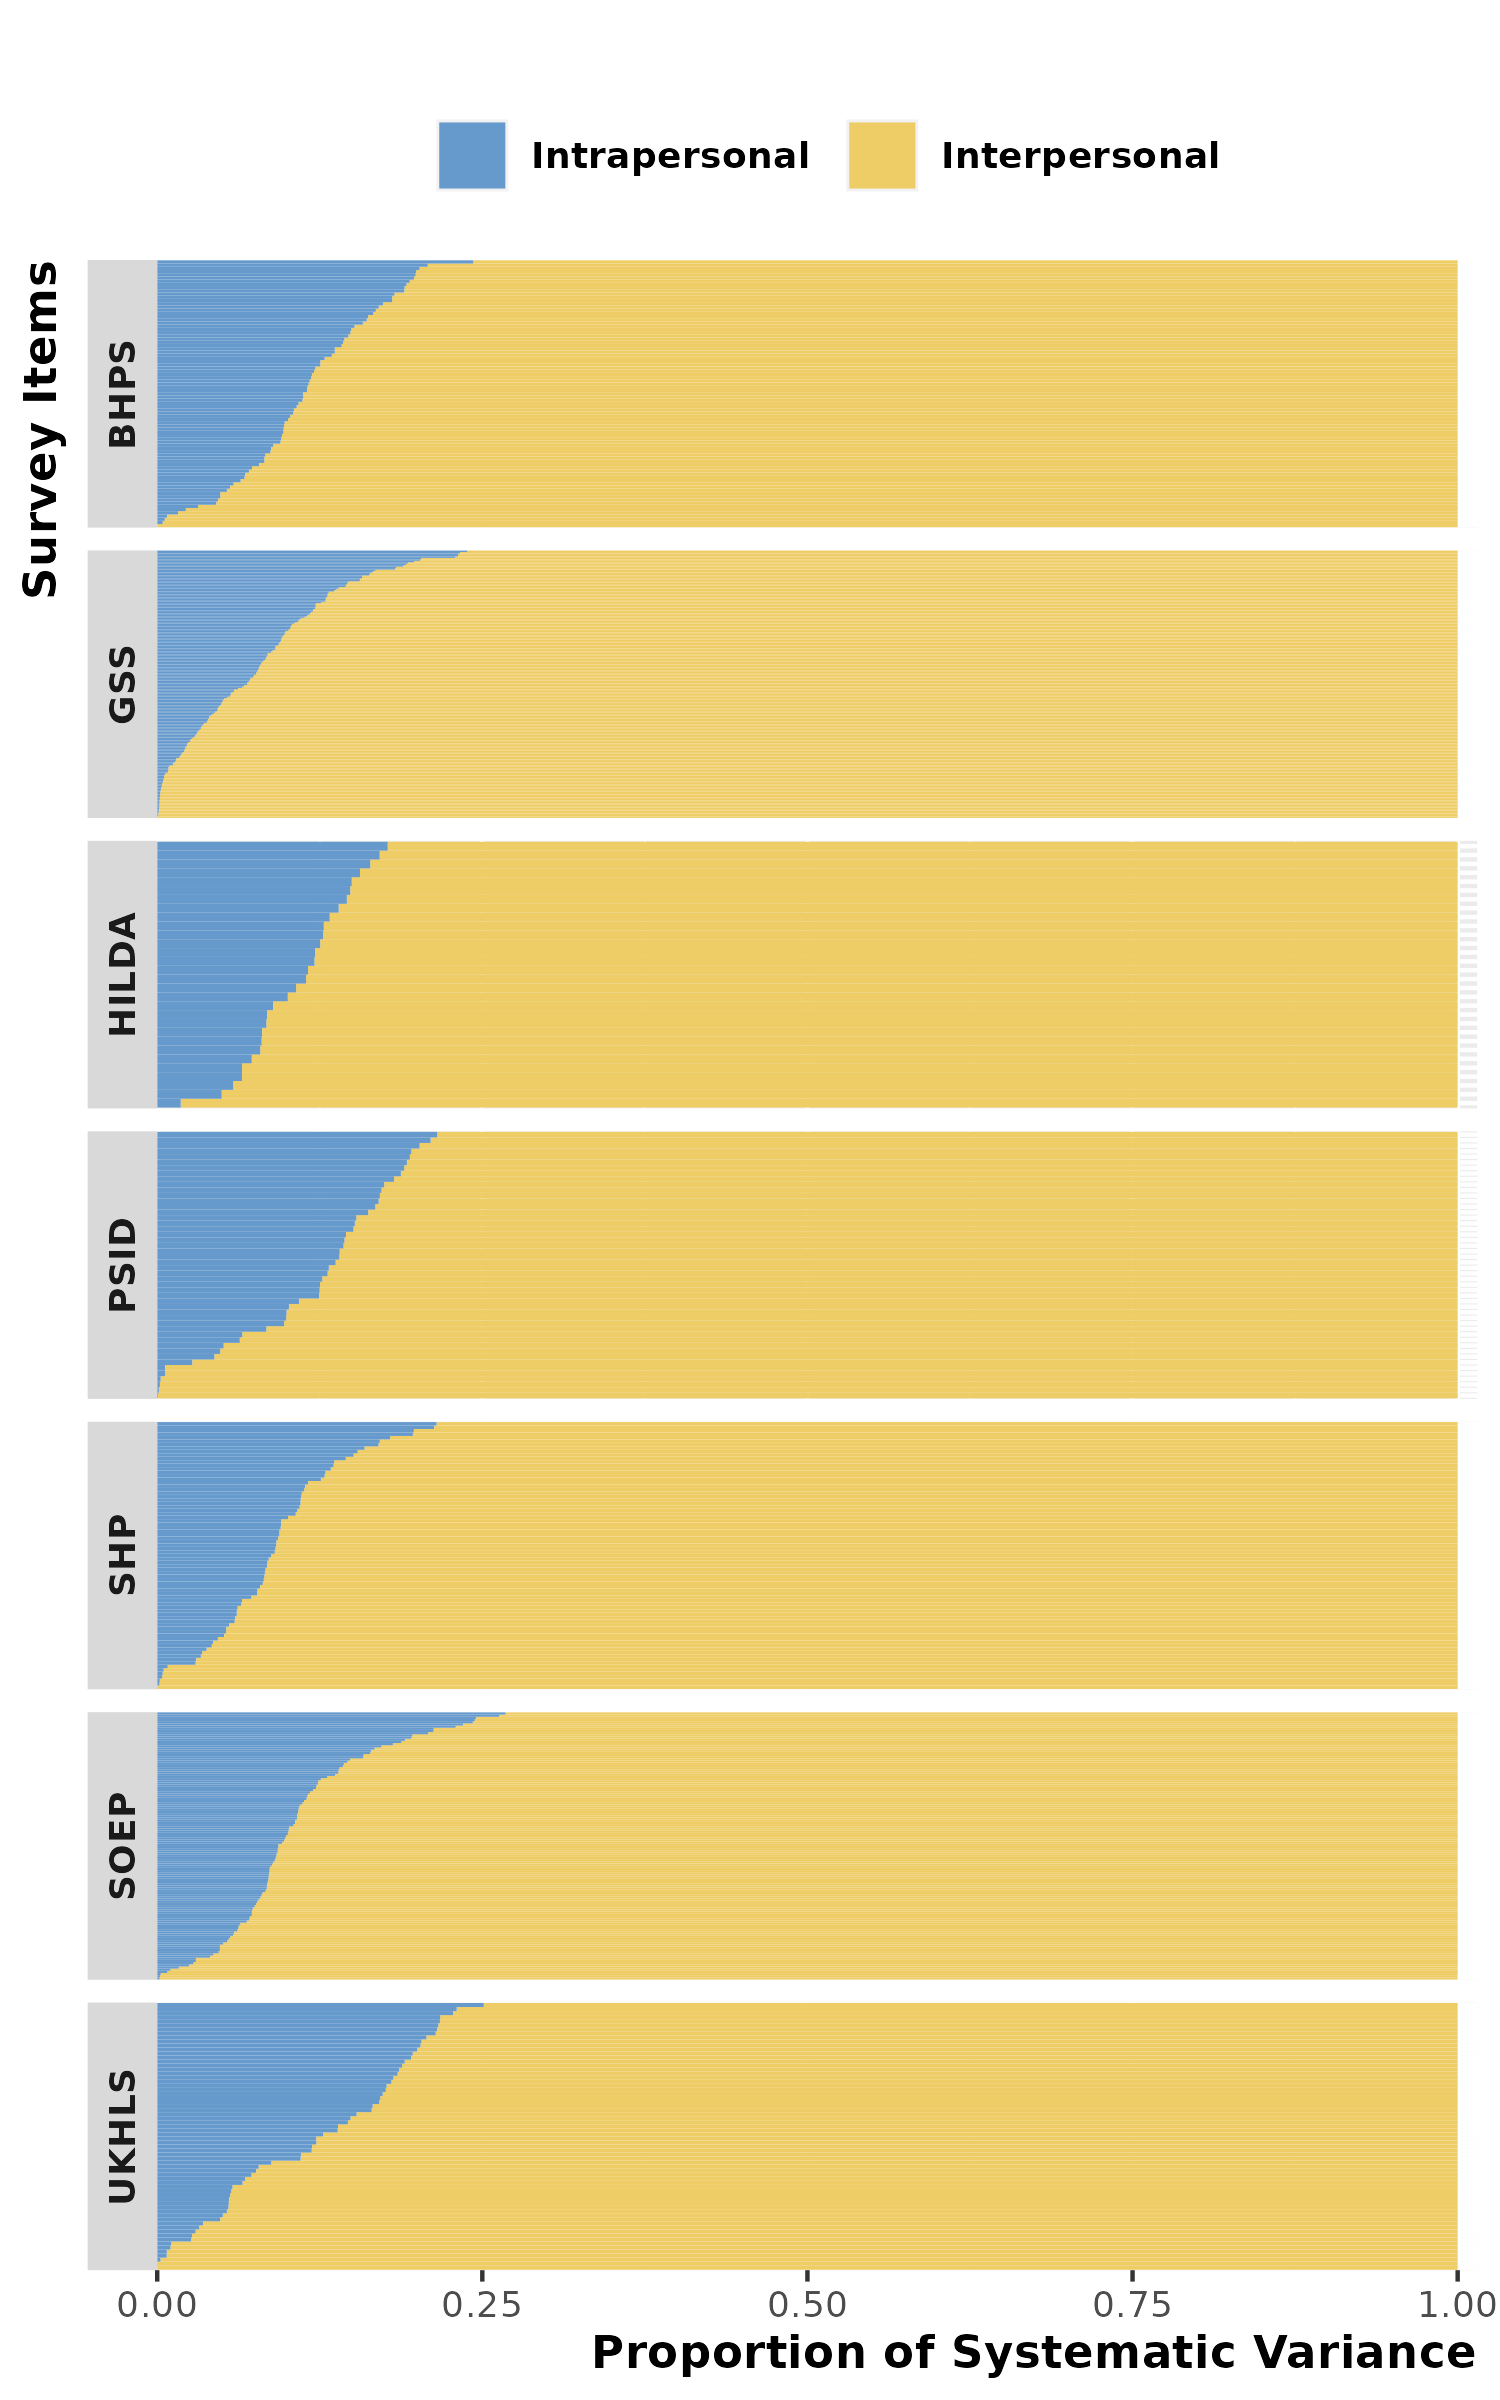
\includegraphics[width=20.71in]{fig/variation_share_lm_mdpnt} 

}

\caption{Proportions of explained variance in items of personal culture; based on predictions at participants' wave mid-point.}\label{fig:fig1}
\end{figure}

\newpage
\begin{figure}

{\centering 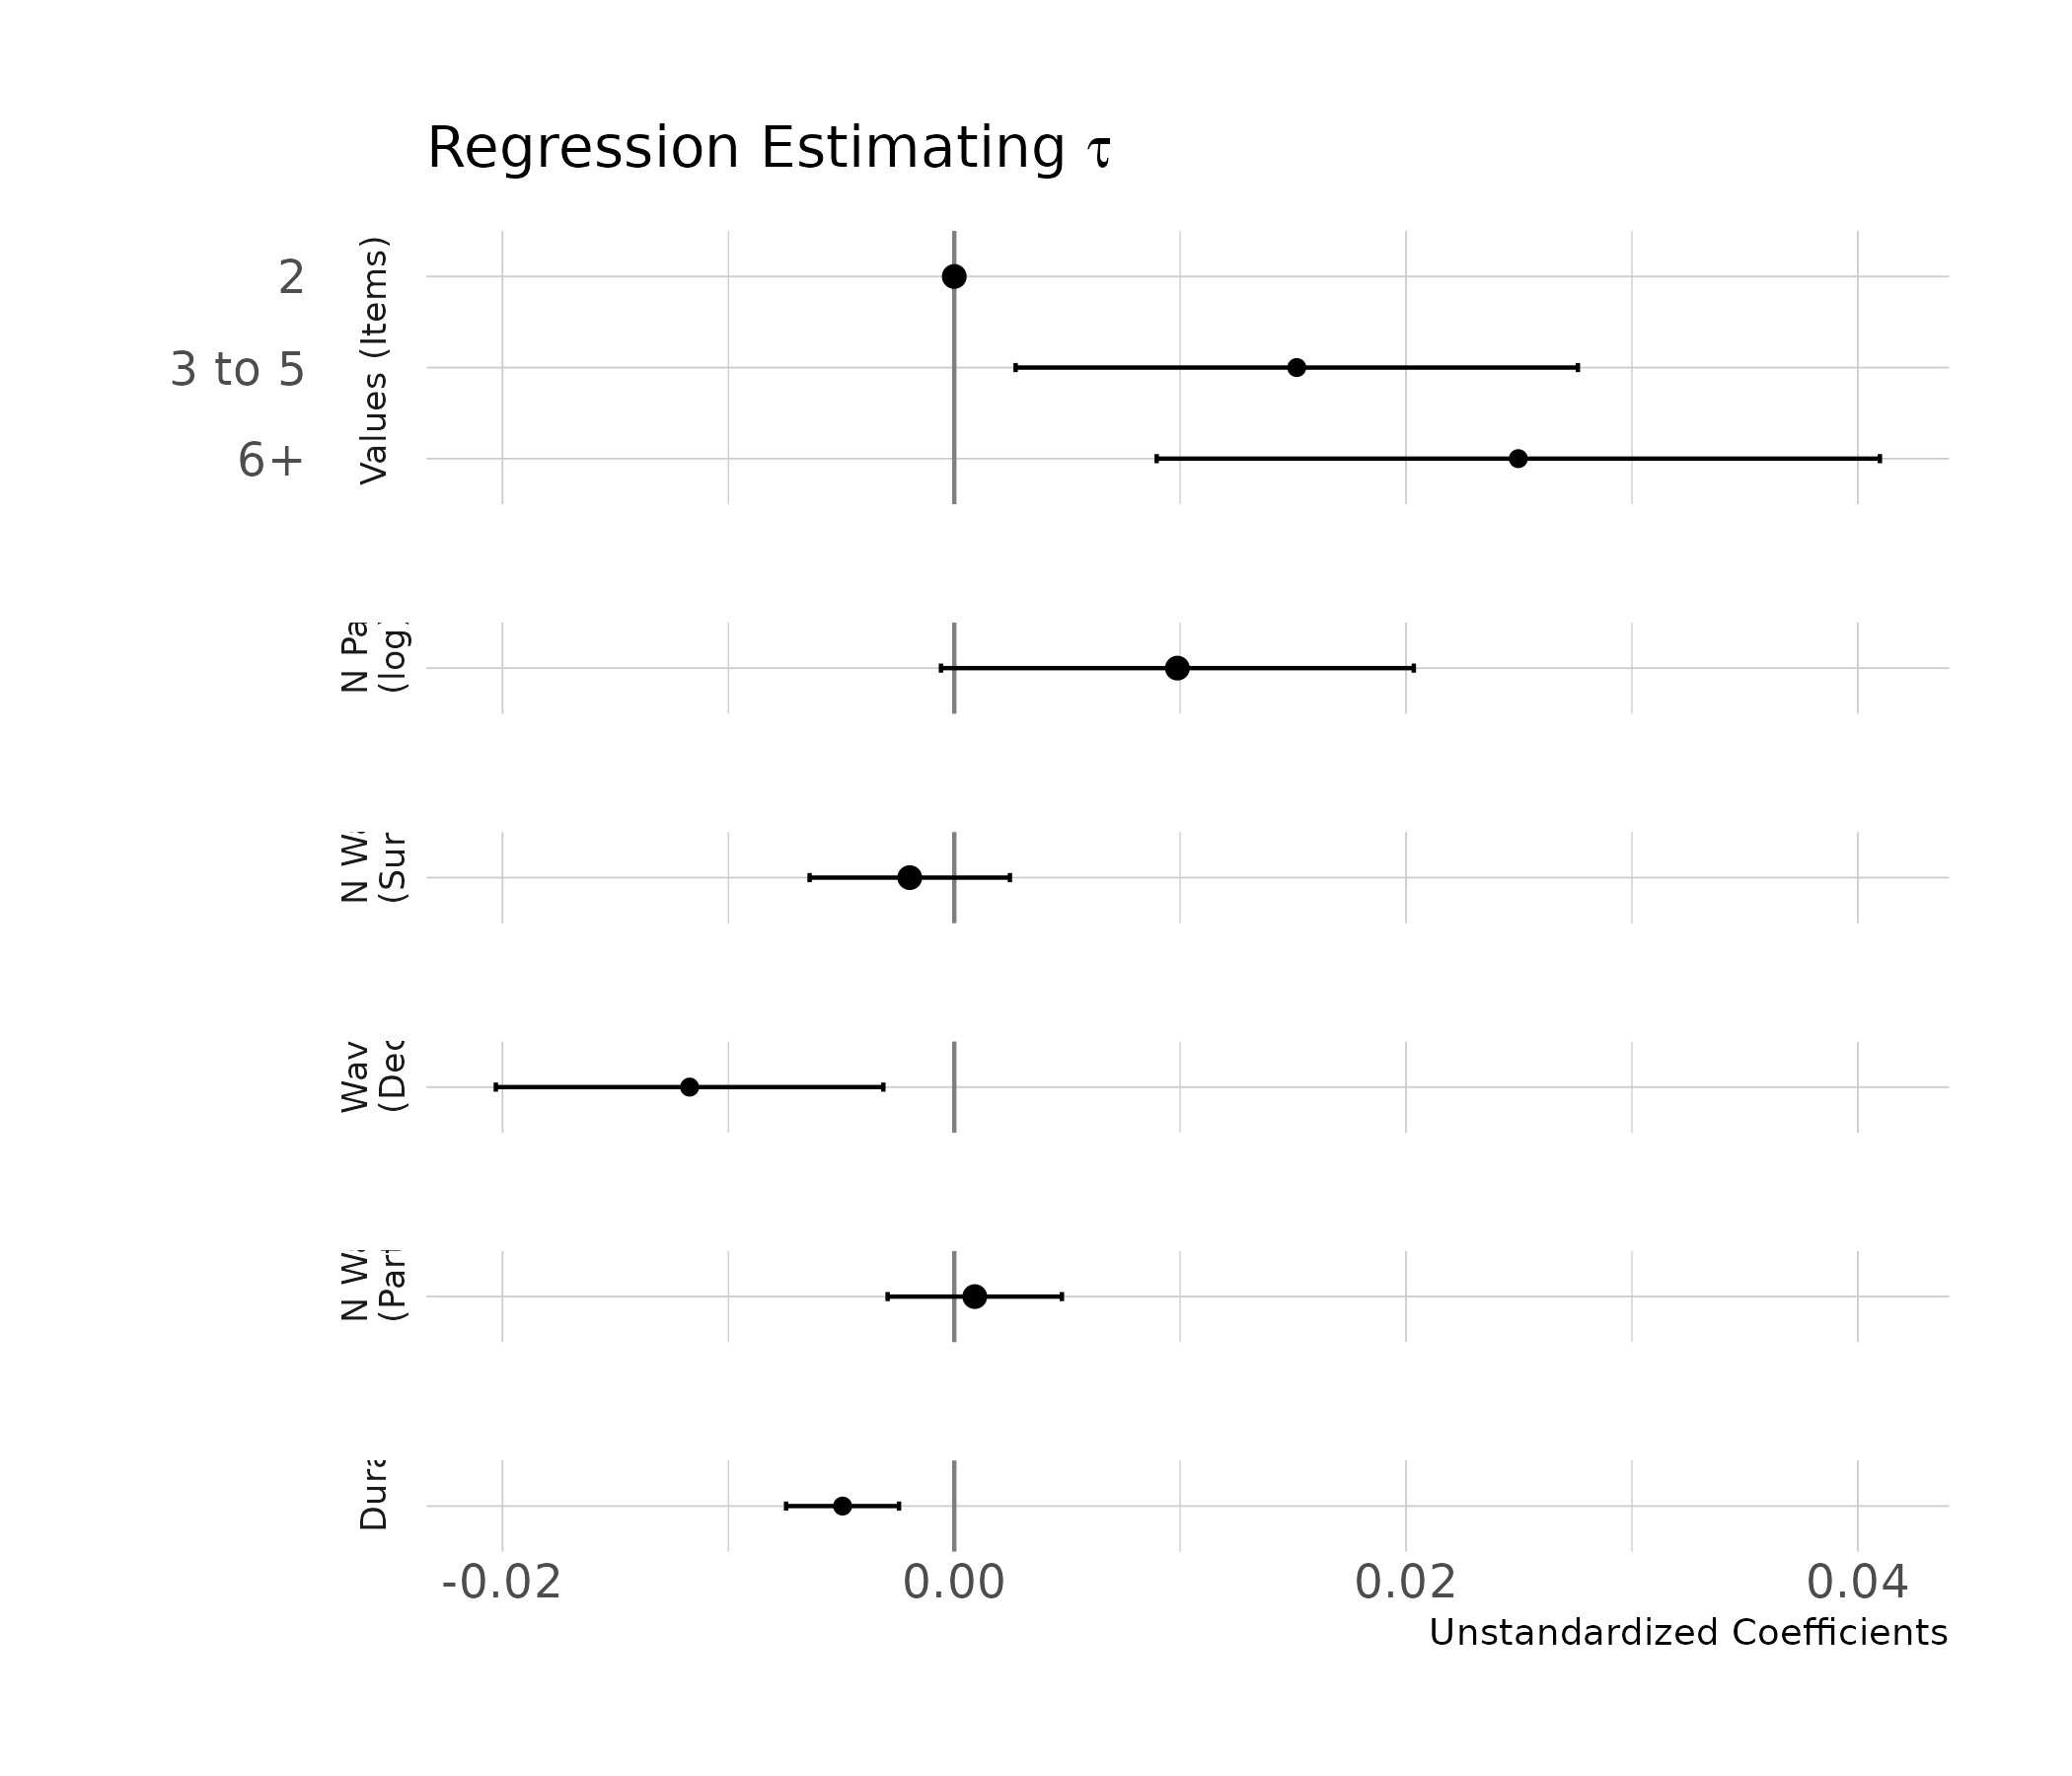
\includegraphics[width=300px]{fig/meta_no_int} 

}

\caption{Proportion of explained variance attributable to intrapersonal change; based on predictions at participants' wave mid-point; supressed intercept model; survey indicators not shown.}\label{fig:fig2}
\end{figure}

\newpage
\begin{figure}

{\centering 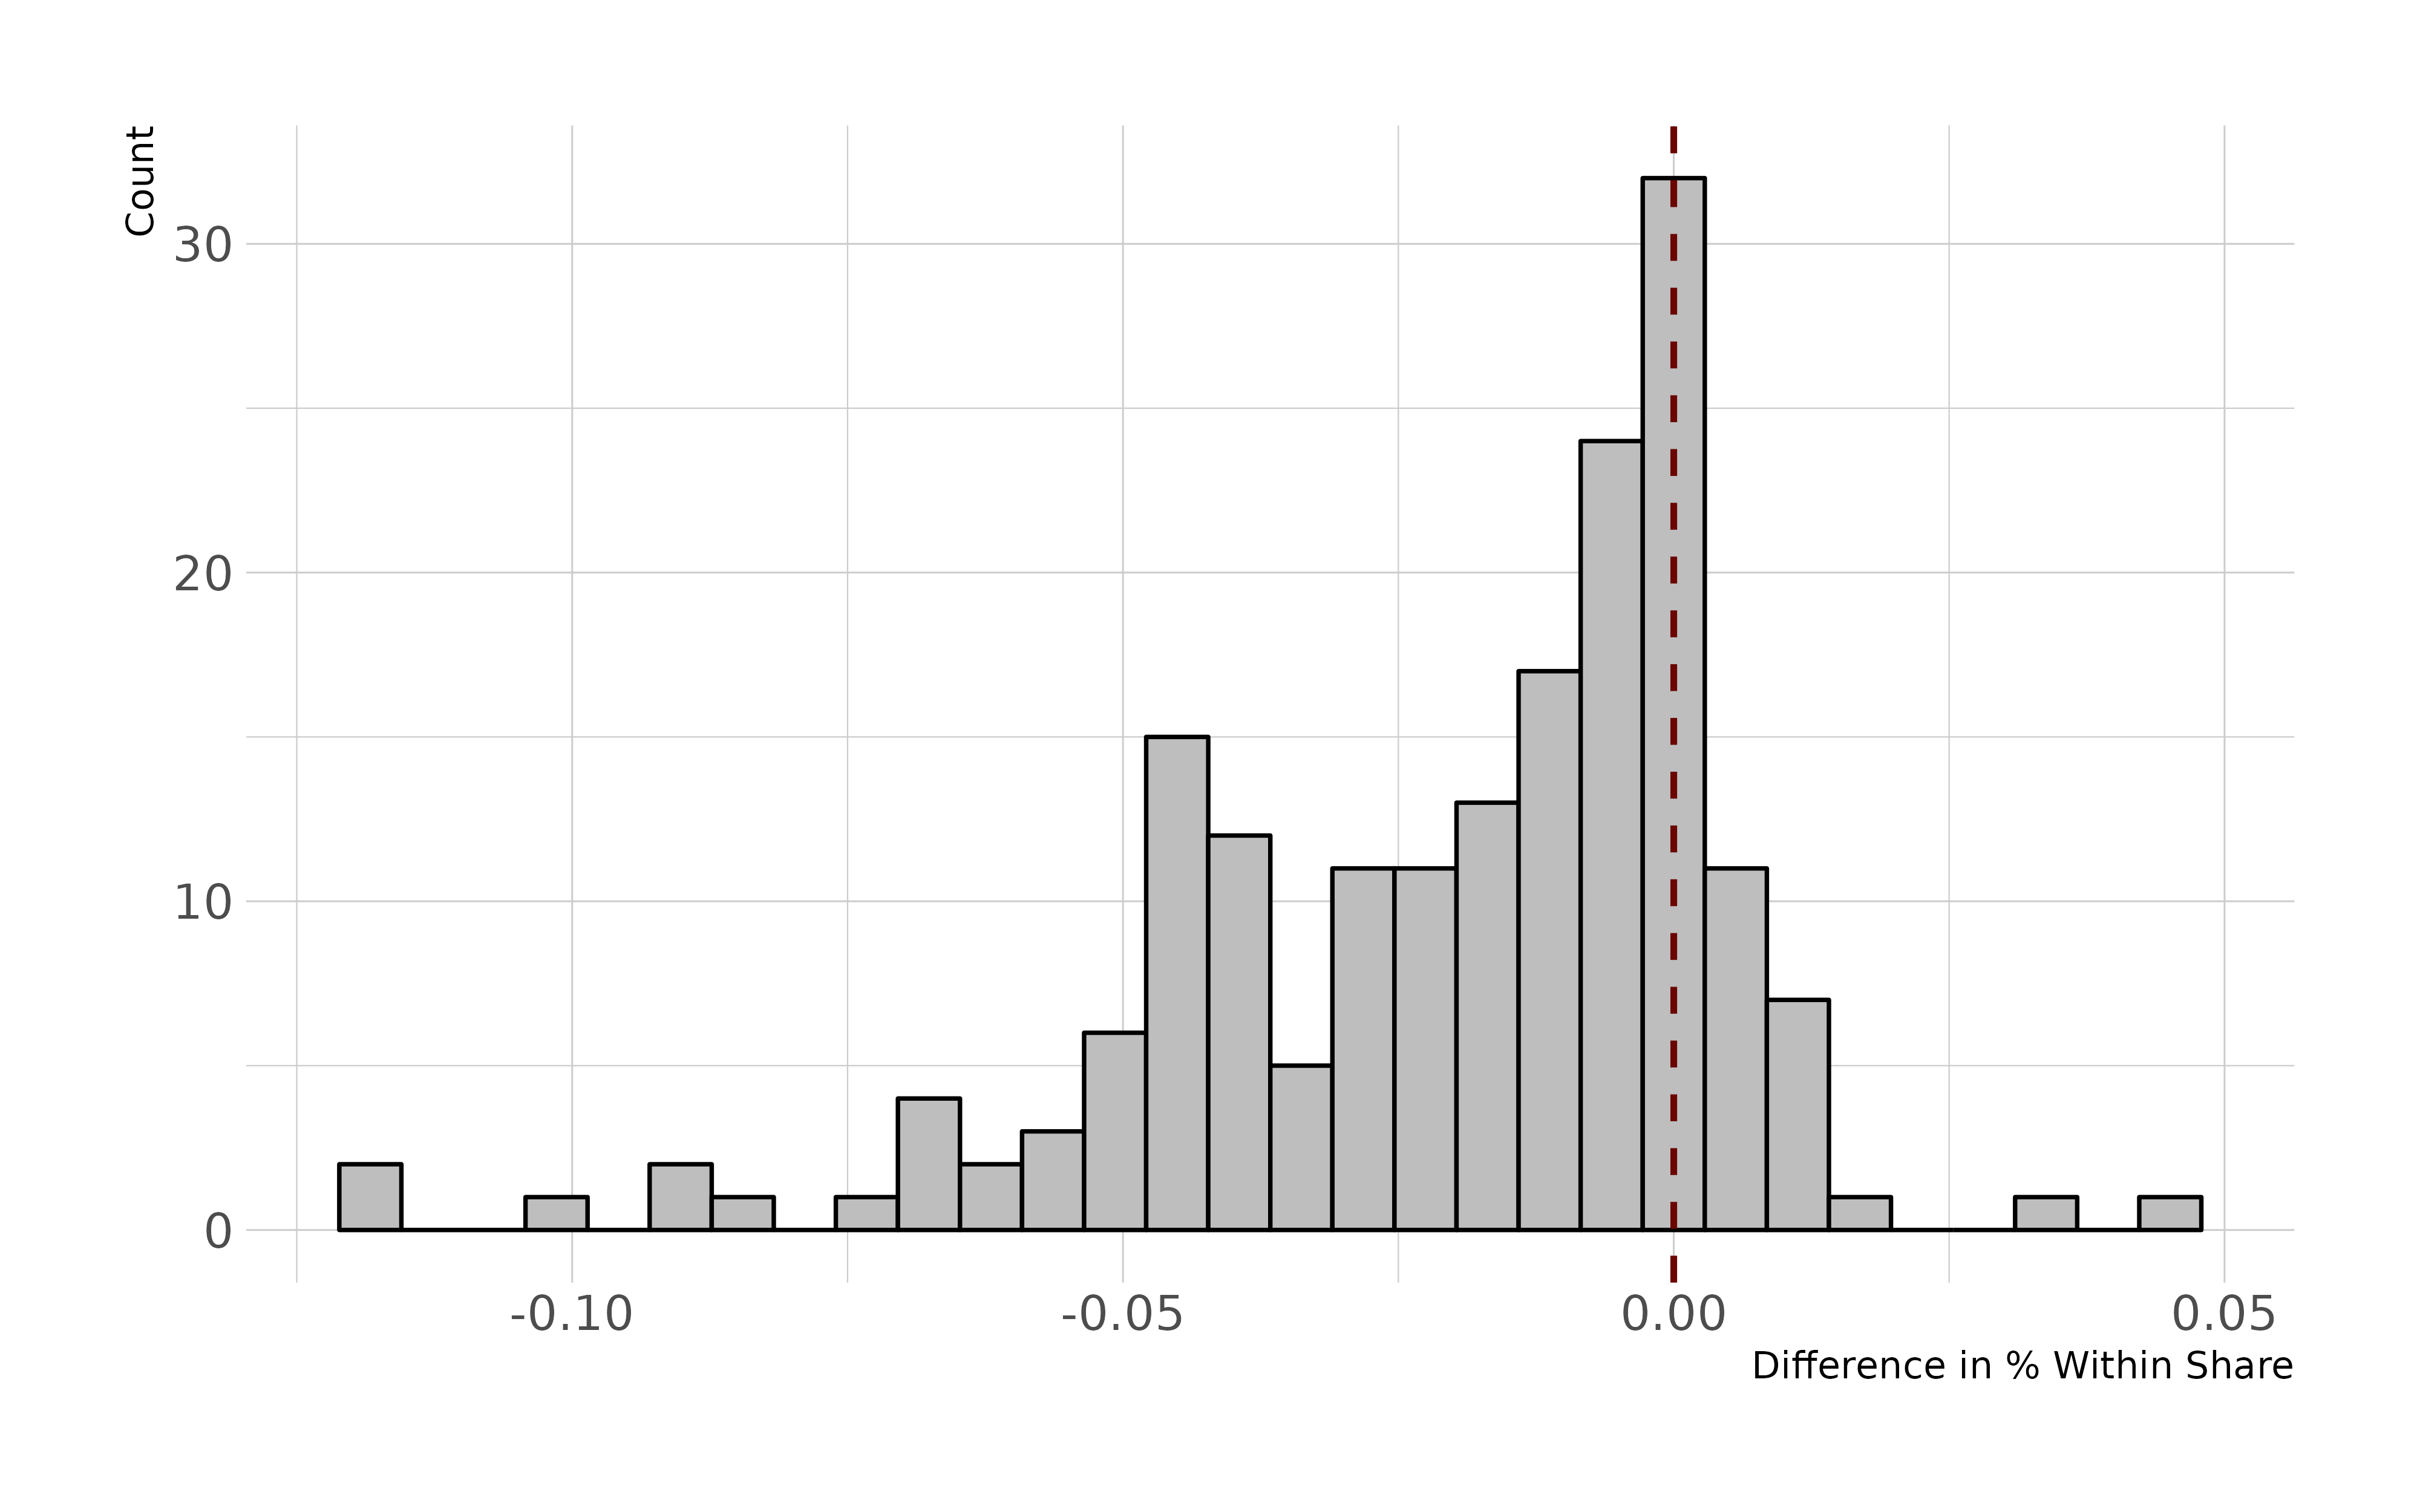
\includegraphics[width=450px]{fig/FIG_college1} 

}

\caption{Figure 3: Distribution of differences share of variance explained by intrapersonal change between respondents without and with college degree.}\label{fig:fig3}
\end{figure}

\newpage
\begin{figure}

{\centering 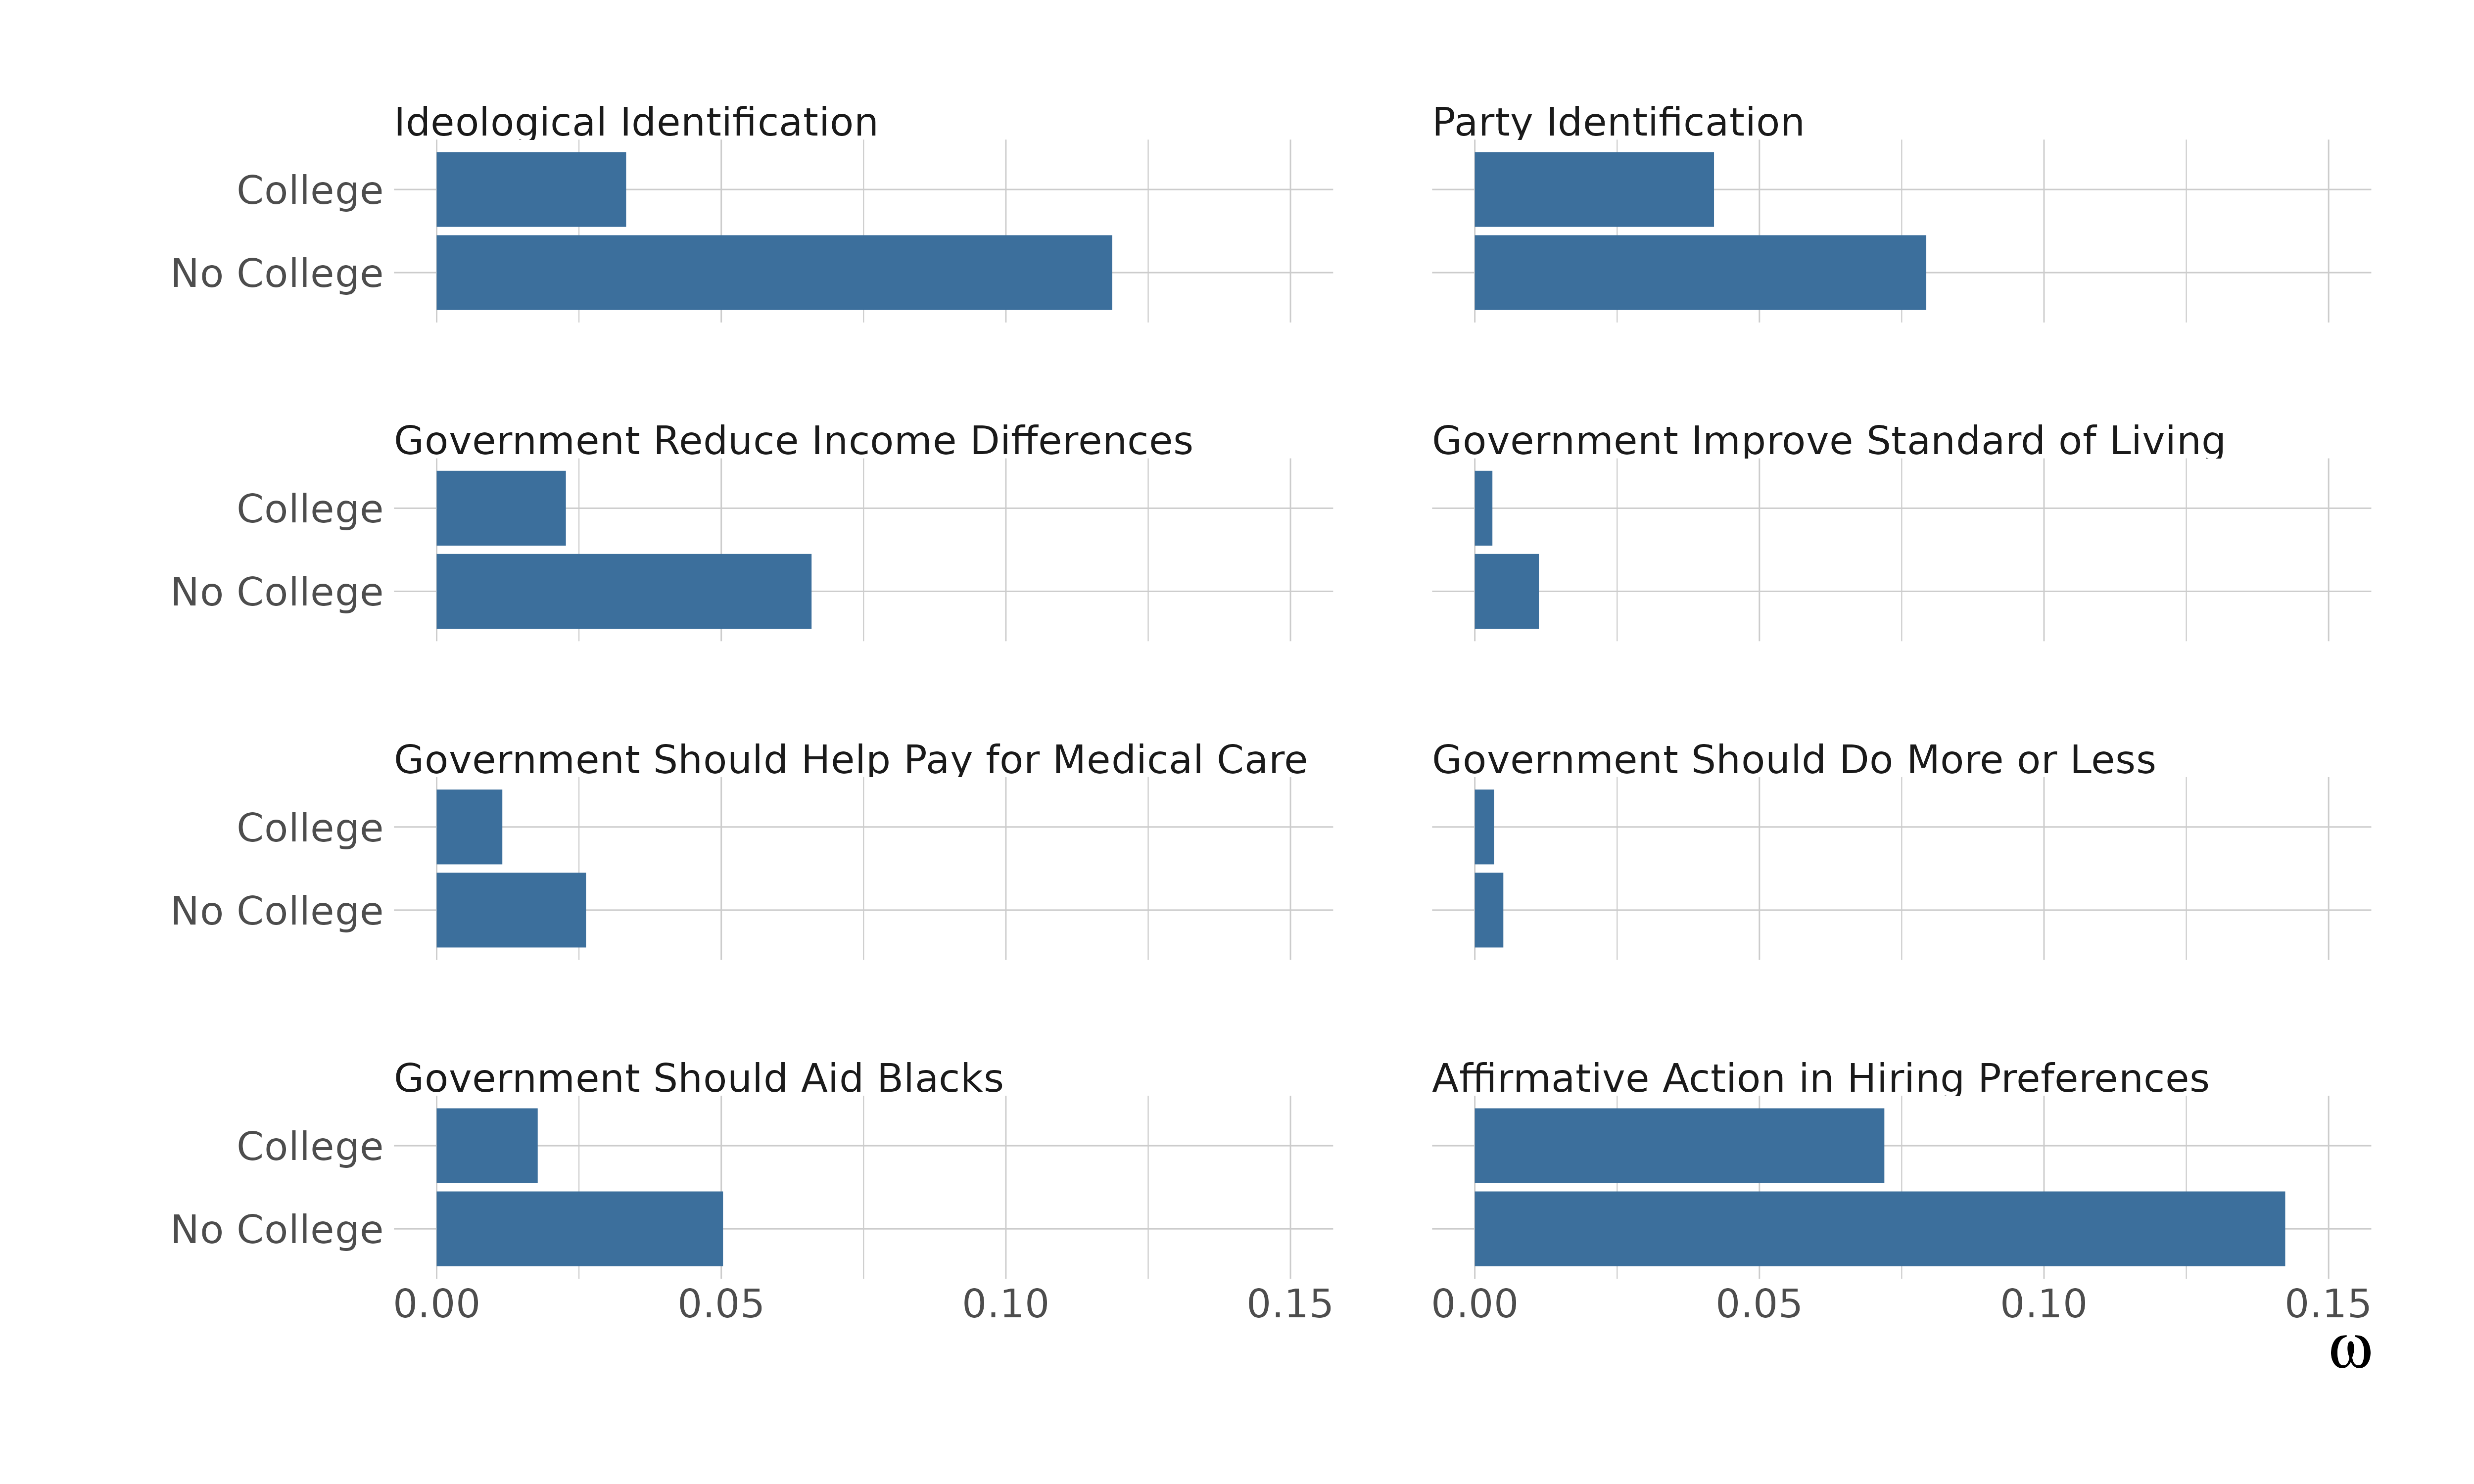
\includegraphics[width=450px]{fig/FIG_college2} 

}

\caption{Proportions of intrapersonal change of explained variance by college degree; based on predictions at participants' wave mid-point.}\label{fig:fig4}
\end{figure}

\end{document}
